\RequirePackage{ifluatex}
\let\ifluatex\relax

\documentclass[aps,%
12pt,%
final,%
oneside,
onecolumn,%
musixtex, %
superscriptaddress,%
centertags]{article} %% 
\topmargin=-40pt
\textheight=650pt
\usepackage[english,russian]{babel}
\usepackage[utf8]{inputenc}
%всякие настройки по желанию%
\usepackage[colorlinks=true,linkcolor=black,unicode=true]{hyperref}
\usepackage{euscript}
\usepackage{supertabular}
\usepackage[pdftex]{graphicx}
\usepackage{amsthm,amssymb, amsmath}
\usepackage{textcomp}
\usepackage[noend]{algorithmic}
\usepackage[ruled]{algorithm}
\usepackage{lipsum}
\usepackage{indentfirst}
\usepackage{babel}
\usepackage{pgfplots}
\usepackage{setspace}
\linespread{1.2}
\pgfplotsset{compat=1.9}
\selectlanguage{russian}
\pgfplotsset{model/.style = {blue, samples = 100}}
\pgfplotsset{experiment/.style = {red}}
\theoremstyle{plain}
\binoppenalty=10000
\newtheorem{theorem}{Теорема}[section] %
\setlength{\parindent}{2.4em}
\setlength{\parskip}{0.1em}
%\renewcommand{\baselinestretch}{1.0}
\theoremstyle{definition}
\newtheorem{definition}{Определение}[subsection]
\theoremstyle{remark}
\newtheorem{remark}{Замечание}[section]

\newtheorem{corollary}{Следствие}
\newtheorem{proposition}{Proposition}
\newtheorem{example}{Пример}
\renewcommand*{\proofname}{Proof}

\newtheorem{lemma}{Лемма}[section]

\graphicspath{ {./image/} }
\usepackage{xcolor}
\usepackage{hyperref}


\begin{document}

\begin{titlepage} 
\begin{center}
% Upper part of the page
%\textbf{\Large САНКТ-ПЕТЕРБУРГСКИЙ ГОСУДАРСТВЕННЫЙ ЭКОНОМИЧЕСКИЙ УНИВЕРСИТЕТ} \\[1.0cm]
%\textbf{\large Кафедра Прикладной Математики и Информатики}\\[3.5cm]
 
% Title
\textbf{}\\[10.0cm]
\textbf{\LARGE Теория игр. Билеты}\\[0.5cm]
\textbf{\Large Александр Широков ПМ-1701} \\[0.2cm]

%supervisor
\begin{center} \large
{Преподаватель:} \\[0.5cm]
\textsc {Чернов Виктор Петрович}\\
\end{center}
% \begin{flushright} \large
%\emph{Рецензент:} \\
%д.ф. - м.н., профессор \textsc{Надеемся Нам Помогут}
%\end{flushright}
%\begin{flushright} \large
%\emph{Заведующий кафедрой:} \\
%д.ф. - м.н., профессор \textsc{Не Обмани Себя}
%\end{flushright}
\vfill 

% Bottom of the page

{\large {Санкт-Петербург}} \par
{\large {2020 г., 6 семестр}}
\end{center} 
\end{titlepage}

% Table of contents
\begin{thebibliography}{3}
  \bibitem{A}
\end{thebibliography}
\tableofcontents
\newpage

\section{Билеты по курсу Теория игра}

\subsection{Понятие игры}

Предметом теории игр является моделированием конфликтных ситуаций. Зачинателем "Теории игр" является Джон фон Нейман, а последователем является Джон Нэш. Зададимся вопросом, а как описать конфликт с помощью математических формул. 

\textbf{Опр:} Cтороны в "конфликте"  называются \textbf{игроками}.

\textbf{Опр}: \textbf{Множество игроков} обозначается как $I$ и каждый игрок принадлежит этому множеству:
$$i \in I \eqno (1)$$ 

\textbf{Опр}: \textbf{Стратегия} в такой игре - правило(отображение), которое преписывает игроку для каждой ситуации в игре ход в это ситуации.

\textbf{Опр}: $S_i$ -\textbf{Множество стратегий}, для каждого игрока $i$ своя стратегия: 
$$ \{S_i\}_{i \in I } \eqno (2)$$

\textbf{Опр}: \textbf{Ситуация} - результат выбора игроками своих стратегий. 

\textbf{Опр}: Размер выигрыша определяется \textbf{платежной функцией} - функция, оценивающая ту или иную ситуацию для отдельного игрока. Данная функция отображает ситуацию в число:
$$ i: \text{ } \{H_i\}_{i \in I } \eqno (3)$$ 
$$ H_{i} (s_1,s_2, ..., s_n) \in \mathbb{R} \eqno (4)$$
т.е каждый игрок оценивает ситуацию вещественным числом.

\textbf{Опр}: Множество игроков, множество стратегий и множество платежных функций называется \textbf{игрой}:
$$ <i \in I, \{S_i\}_{i \in I },\{H_i\}_{i \in I } > \eqno (5)$$
 
\textbf{Пример:} на столе лежит $100$ камешков, играют два человека. Ход состоит в том, что каждый игрок забирает из кучки от $1$ до $5$ камешкев по своему усмотрению. Тот, кто взял последним, выиграл. Существуют ли выигрышные стратегии для игроков?

\begin{proof}
  Первый ход: берем 4 камня, а после дополняем количество камешкев до 6. Первый выигрывает.
\end{proof}

\newpage
\subsection{Формы задания игр. Представление игры в древовидной и матричной форме. Антагонистические игры. Решение игры}

\textbf{Древовидная форма}

Для каждой из игр строится \textbf{дерево игры}, состоящее из стратегий, где каждая \textbf{ветвь} - отдельная игра, а \textbf{узлы} данного вида - ситуации.

\textbf{Матричная форма}

На основе дерева игры попытаемся создать \textit{матрицу данной игры} размером $m \times n$ Количество \textit{строк} в данной матрице $m$ - \textit{количество стратегий} первого игрока, количество \textit{столбцов} $n$ - количество стратегий второго игрока. 

Первый игрок выбирает какую-то строку этой матрицы, второй - какой-то столбец, другими словами первый игрок выбирает какую-то стратегию, а на пересечении столбцов и строк находится размер выигрыша первого игрока (при нулевом балансе у проигравшего получается $-1$, а у выигрывшего $1$).

Пусть $H_1$ - матрица выигрыша первого игрока, $H_2$ - матрица выигрыша второго игрока и сумма элементов на одинаковых позициях в этих таблицах равна нулю.

\textbf{Антагонистические игры}

\textbf{Опр}: Если сумма платежных функций (матриц функций) равна нулю, то такая игра называется игрой с \textit{нулевой суммой}.
$$\sum_{i \in I}{H_{i} (s_1,s_2, ..., s_n) = 0} \eqno (6)$$ 

\textbf{Опр}: Если сумма равна какой-то константе, то такая игра называется игрой с \textit{постоянной суммой}.
$$\sum_{i \in I}{H_{i} (s_1,s_2, ..., s_n) = Const} \eqno (7)$$ 

\textbf{Опр}: \textit{антагонистическая игра} - игра двух игроков с нулевой суммой. В такой игре если выигрывает один, то обязательно проигрывает другой, то есть это игра, в которой выигрыш одного из игроков точно равен проигрышу другого.

Так как сумма матриц равна нулю, то: 
$$H_1 = -H_2 \eqno (8)$$

следовательно, нам не нужно две матрицы и будем проводить рассуждение на основе матрицы выигрышей первого игрока.

\textbf{Опр:} \textbf{Смоделировать} (решить) антагонистическую игру - значит, для каждого игрока указать стратегии, \textbf{удовлетворяющие условию оптимальности}, т.е. игрок A должен получить максимальный гарантированный выигрыш, какой бы своей стратегии не придерживался игрок B, а игрок B должен получить минимальный проигрыш, какой бы своей стратегии не придерживался игрок A. 

\textbf{Опр:} \textbf{решением игры} является пара оптимальных стратегий для игроков, а также в ряде классов игр определение \textit{цены игры}. Оптимальные стратегии обладают тем свойством, что если один из игроков придерживается своей оптимальной стратегии, то другому не может быть выгодно отступать от своей.

\newpage
\subsection{Неравенство минимаксов}

Рассмотрим матрицу $ A_{m \times n}$ с элементами , являющимися вещественными числам, для антагонистической игры, в которую играют два игрока. Первый игрок выбирает номер строки, а второй игрок выбирает номер столбца. 

То, что находится на пересечении $(a_{ij})$ - размер выигрыша(проигрыша) игрока первого игрока, $(-a_{ij})$ - проигрыша(выигрыша) второго игрока.

Будем выписывать минимальные элементы по строке: 
$$ \underset{j}{\min} = \{a_{1,j_1}, ... , a_{m,j_m}\} \eqno (9)$$

\textbf{Опр}: Среди данных минимумов выберем $\max$ среди $\min$. Данная величина называется \textit{максимином}:
$$ \underset{i}{\max} (\text{ } \underset{j}{\min} \text{ } a_{ij}) = a_{i_{0},j_{0}} \eqno (10)$$

То есть в самой худшей ситуации, если он выберет эту строку, то это будет минимальным его выигрышем. Также данную величину называют \textbf{нижней ценой игры}.

Допустим второй игрок выбирает первый столбец, тогда худшим вариантом для него будет максимум по строкам в каждом столбце:

$$ \underset{i}{\max} = \{a_{i_1,1}, ... , a_{i_n,n}\} \eqno (11)$$

\textbf{Опр}: Среди данных минимумов выберем $\min$ среди $\max$ (лучшее среди худшего). Данная величина называется \textit{минимаксом}:
$$ \underset{j}{\min} (\text{ }\underset{i}{\max} \text{ } a_{ij}) = a_{i_1,j_1} \eqno (12)$$

Получили гарантированный проигрыш второго игрока. 

Также данную величину называют \textbf{верхней ценой игры}.

Предположим, что эти элементы совпали, тогда такой элемент называется седловой точкой.

%\textbf{Опр}: седловой точкой называется точка, для которой $a_{i_0,j_0} = a_{i_1,j_1}$, являющаяся минимумом по одной оси, и точка максимума по другой.

\textbf{Опр}: \textbf{Седловой точкой} называется точка(элемент матрицы), которая является минимальным в своей строке и максимальной в своем столбце. В этом случае значение верхней цены игры равно значению нижней цены игры и значение минимакса и максимина называется \textbf{ценой игры}.

\textbf{Опр}: \textbf{Устойчивая ситуация} - ситуация, из которой невыгодно выходить любому игроку. Признак решения конфликта - наличие свойства устойчивости. 

Такое решение называется решением по \textbf{Нэшу}.

Оптимальные стратегии характеризуются устойчивостью, то есть ни одному из игроков не выгодно отклоняться от своей оптимальной стратегии.

\begin{theorem} 
  Неравенство максимина и минимакса

  Дана матрица $A_{m \times n}$ и $a_{ij}$ - элементы матрицы. 

  Рассмотрим максимин и минимакс: $a_{pq}$ и $a_{rs}$, такие, что:
  $$ a_{pq} = \underset{i}{\max} \text{ } (\underset{j}{\min} \text{ } a_{ij}) \eqno (13)$$
  $$ a_{rs} = \underset{j}{\min} \text{ } (\underset{i}{\max} \text{ } a_{ij}) \eqno (14)$$

  Тогда $$a_{pq} \leq a_{rs} \eqno (15)$$
\end{theorem}
\begin{proof}
  Рассмотрим матрицу и рассмотренные в ней элементы $a_{pq}$ и $ a_{rs}$.
  $$\begin{pmatrix}
   \cdot  & \cdot &  \cdot  & \cdot  & \cdot \\ 
   \cdot &a_{pq} & \cdot  &a_{ps} & \cdot \\ 
   \cdot  & \cdot  & \cdot  & \cdot  & \cdot \\ 
   \cdot & \cdot & \cdot & a_{rs} &  \cdot \\ 
   \cdot & \cdot & \cdot & \cdot & \cdot 
  \end{pmatrix}$$

  Пусть рассматривается $a_{ps}$ - элемент матрицы $A_{m \times n}$.
  $a_{ps} \leq a_{rs}$, так как $a_{rs}$ - максимум в столбце. 

  С другой стороны $a_{pq}$ - минимум в строке, следовательно $a_{pq} \leq a_{ps}$. Тогда из двух неравенств получаем: $a_{pq} \leq a_{ps} \leq a_{rs}$.
\end{proof}

\newpage
\subsection{Теорема о седловой точки}

Рассмотрим теперь теорему и необходимом и достаточном условии седловой точке в матрице.

\begin{theorem} 
  Необходимое и достаточное условие седловой точки

  Чтобы задача имела седловую точку необходимо и достаточно, чтобы $$a_{pq} = a_{rs} \eqno (16) $$
\end{theorem}

\begin{proof}
  1. $\exists$  седловая чтока $\Rightarrow a_{pq} = a_{rs}$. Пусть $ a_{kl}$ - седловая точка.
  $$\begin{pmatrix}
  \cdot  & \cdot &  \cdot &  \cdot  & \cdot \\ 
  \cdot &a_{pq} & \cdot  & \cdot  & \cdot \\ 
  \cdot  & \cdot  & a_{kl} &  a_{ks} &  \cdot \\ 
  \cdot & \cdot  &  \cdot & a_{rs} &  \cdot \\ 
  \cdot & \cdot  &  \cdot  &   \cdot    &  \cdot 
  \end{pmatrix}$$

  Если бы мы писали строку максимумов, то в ней бы были точки $a_{kl},..., a_{rs}$, но в этой строке $a_{rs}$ является минимумом, следовательно: $$ a_{kl} \geq a_{rs} $$

  Если бы мы писали столбец минимумов, то в ней бы были точки $a_{pq},..., a_{kl}$, но в этом столбце $a_{pq}$ является максимумом, следовательно: 
  $$ a_{pq} \geq a_{kl}$$

  Из двух неравенств получаем следующие соотношения:
  $$ a_{pq} \geq a_{kl} \geq a_{rs} $$
  $$ a_{pq} \geq a_{rs} $$

  Но по формуле (15):
  $$ a_{pq} \leq a_{rs} $$

  Следовательно:
  $$ a_{pq} = a_{rs} $$

  Необходимость доказана

  2. $a_{pq} = a_{rs}$  $\Rightarrow $ Нужно доказать, что $\exists$ - седловая точка. 

  Для доказательства обратного случая нужно построить каким-то образом седловую точку. Выберем точку $a_{ps}$, как показано ниже, и докажем, что данная точка является седловой. 
  $$\begin{pmatrix}
  \cdot  &  \cdot &   \cdot &   \cdot  &  \cdot \\ 
  \cdot &a_{pq} &  \cdot  & a_{ps}  &  \cdot\\ 
  \cdot  &  \cdot  &  \cdot &   \cdot &   \cdot \\ 
  \cdot &  \cdot  &   \cdot & a_{rs} & \cdot \\ 
  \cdot &  \cdot  &   \cdot  &    \cdot    &   \cdot
  \end{pmatrix}$$
  $$a_{pq} \leq a_{ps} \leq a_{rs}$$

  Можно записать как равенство, так как по условию достаточности:
  $$ a_{pq} = a_{ps} = a_{rs}$$

  Этот элемент равен минимальному в строке и максимальному в столбце - определение минимакса и максимина $\underset{\text{def}}{\Rightarrow}$ седловая точка. 
\end{proof}

\subsubsection{Прямоугольность множества седловых точек. Единственность цены игры.}

\begin{theorem}
  Множество седловых точек

  Пусть $a_{kl}$ и $a_{uv}$ - седловые точки, тогда $a_{kv}$ и $a_{ul}$ - тоже седловые точки. 
\end{theorem}

\begin{proof}
  $$\begin{pmatrix}
  \cdot  &  \cdot &   \cdot &   \cdot  &  \cdot \\ 
  \cdot &a_{kl} &  \cdot  & a_{kv}  &  \cdot \\ 
  \cdot  &  \cdot  &  \cdot &   \cdot &   \cdot \\ 
  \cdot & a_{ul}  &   \cdot & a_{uv} & \cdot \\ 
  \cdot &  \cdot  &   \cdot  &    \cdot    &   \cdot 
  \end{pmatrix}$$
  $$ a_{kl} \geq a_{ul} \geq a_{uv} \geq a_{kv} \geq a_{kl} $$

  Так как концы равны, то можно заменить равенствами. 
  $$ a_{kl} =a_{ul} = a_{uv} = a_{kv} = a_{kl} $$

  Следовательно, $a_{ul}$ и $a_{kv}$ - максимальный в своем столбце и минимальный в своем столбце $\underset{\text{def}}{\Rightarrow}$ седловые точки.
\end{proof}

\textbf{Замечание:} все седловые точки \textit{равны друг другу}, следовательно \textbf{цена игры единственна}.

\textbf{Замечание:} если элемент матрицы \textit{равен седловой точке}, то он \textit{не обязательно является седловой точкой}.

Рассмотрим пример:
$$
\begin{pmatrix}
1_{s} & 1_{s} \\
0 & 1 \\
\end{pmatrix}
$$

В данном примере в первой строке являются седловыми точками, но единица во второй строке не седловая точка, хоть и равна ей.

\newpage
\subsection{Алгоритм нахождения седловой точки. Организация поиска седловой точки средствам Excel}
Будем рассматривать переменные на прямоугольнике.

Пусть задана функция $f(x.y)$ и играется в антоганистическую игру двумя соперниками. 
Первый игрок выбирает значение $x$ на своем промежутке $x:a \leq x \leq b$, а второй игрок выбирает какое-то значение $y: c \leq y \leq d$. 

\textbf{Алгоритм нахождения седловой точки:}

\begin{enumerate}
  \item $ \underset{x}{\max} \text{ }\underset{y}{\min} \text{ }  f(x,y) $
  \begin{enumerate}
    \item $ \underset{y}{\min} \text{ } f(x,y) = g(x) $
    \item $ \underset{x}{\max} \text{ } g(x) = A $
  \end{enumerate}
  \item $ \underset{y}{\min} \text{ }\underset{x}{\max} \text{ }  f(x,y) $
  \begin{enumerate}
    \item $ \underset{x}{\max} \text{ } f(x,y) = h(y) $
    \item $ \underset{y}{\min} \text{ } h(y) = B $
  \end{enumerate}
  \item $A = B ?$
\end{enumerate}

\subsubsection{Решение задач на нахождение седловой точки}

\textbf{Задача 1:}

Проверить, есть ли у функции седловая точка.
$$ f(x,y) = (x-y)^2 $$
$$ -1 \leq x \leq 1,-1 \leq y \leq 1 $$
Покажем, что седловой точки нет у данной функции.

\begin{proof}
  Найдем максимин:
  $$ \underset{y}{\min} \text{ } f(x,y) = (f(x,y))_y'  = -2x + 2y = g(x)$$
  $$ y = x $$
  $$ A = \underset{x}{\max} \text{ } g(x) = 0 $$

  Найдем минимакс:
  $$ \underset{x}{\max} \text{ } f(x,y) = (f(x,y))_x'  = 2x -  2y = h(y) \Rightarrow x = y$$

  При каждом y свое значение максимума:

  Исследуем границы:
  $$ \max (1-y)^2 = 4 \text{ ;  } \max (-1-y)^2 = 4 $$
  $$h(y) = \left\{\begin{matrix}
  (1-y)^2, -1 \leq y \leq 0\\ 
  (1+y)^2, 0 \leq y \leq 1
  \end{matrix}\right.$$
  $$ B = \underset{y}{\min} \text{ } h(y) = 1 $$

  Седловой точки нет, так как $A \neq B$
\end{proof}

\textbf{Задача 2:}
$$ f(x,y) = (x-y)^2 - 0.5y $$
$$ -1 \leq x \leq 1,-1 \leq y \leq 1 $$

Покажем, что седловой точки нет у данной функции.
\begin{proof}
  В общем случае, нет стационарной точки, значит будем искать на границах.

  Найдем максимин:
  $$ \underset{y}{\min} \text{ } f(x,y) = (f(x,y))_y'  = -2x + 2y -0.5 = g(x)$$
  $$(f(x,y))_y'' = 2  -\text{точка минимума}$$ 
  $$ y = x + 0.25$$

  Из трех функций нужно было бы найти min среди трех выражений $f(x,1),f(x,-1),-0.0625x$
  $$g(x) = \max{f(x,1),f(x,-1),f(x,x+0.25)}$$
  $$ g(x) = -0.0625 - 0.5 x,\quad  x\to -1 $$
  $$ A = \underset{x}{\max} \text{ } g(x) = 0.4375 $$

  Найдем минимакс:
  $$ \underset{x}{\max} \text{ } f(x,y) = (f(x,y))_x'  = 2x -  2y = h(y) \Rightarrow x = y$$

  При каждом y свое значение максимума:

  Исследуем границы:
  $$ \max (1-y)^2 = 4 \text{ ;  } \max (-1-y)^2 = 4 $$
  $$h(y) = \left\{\begin{matrix}
  (1-y)^2, -1 \leq y \leq 0\\ 
  (1+y)^2, 0 \leq y \leq 1
  \end{matrix}\right.$$
  $$ B = \underset{y}{\min} \text{ } h(y) = 1 $$

  Седловой точки нет, так как $A \neq B$
\end{proof}

\textbf{Задача 3:}

$$ f(x,y) = (x-y(1-y^2))^2 = x^2 - 2 x y + y^2 + 2 x y^3 - 2 y^4 + y^6$$
$$ -1 \leq x \leq 1,-1 \leq y \leq 1 $$

Покажем, что седловой точки нет у этой функции.
\begin{proof}
  Обозначим за $y(1-y^2) = u$, тогда получим функцию: $f(x,u) = (x-u)^2$

  Для того, чтобы узнать границы, найдем минимум и максимум функции $u$:
  $$ \min (y - y^3) =-\frac{2}{3\sqrt3}$$
  $$ \max (y - y^3) = \frac{2}{3\sqrt3}$$

  1. Найдем максимин:
  $$ \underset{u}{\min} \text{ } f(x,u) = (f(x,u))_u'  = -2(x-u) - \text{точка минимума}$$
  $$u=x$$
  $$g(x) = \left \{
  \begin{matrix}
  (x+\frac{2}{3\sqrt3})^2 \quad -1 \leq x \leq -\frac{2}{3\sqrt3} \\
  {}\\
    0 \qquad -\frac{2}{3\sqrt3} \leq x \leq \frac{2}{3\sqrt3} \\
  {} \\
  (x-\frac{2}{3\sqrt3})^2 \quad \frac{2}{3\sqrt3 } \leq x \leq 1
  \end{matrix}\right.$$
  $$ A = \underset{x}{\max} \text{ } g(x) = \left (1 - \frac{2}{3\sqrt {3}}\right)^2$$

  2. Найдем минимакс:
  $$ \underset{x}{\max} \text{ } f(x,u) = (f(x,u))_x'  = 2x -  2u = h(u) \Rightarrow x = u$$

  Исследуем границы:
  $$h(u) = \left\{
  \begin{matrix}
  (1+u)^2,\frac{2}{3\sqrt{3}}\geq u \geq 0 \\ 
  (1-u)^2, -\frac{2}{3\sqrt{3}}\leq u \leq 0
  \end{matrix}\right.$$

  Рисуем график и находим минимум.
  $$ B = \underset{u}{\min} \text{ } h(u) = 1$$

  Седловой точки нет, так как $A \neq B$.
\end{proof}

\subsubsection{Организация поиска седловой точки средствам Excel}

Реализация данного метода построенна на представлении значения функции с помощью сетки с определенным шагом и проверки необходимого и достаточного условия седловой точки.

Решение приведено в файле:
$$\textsc{1. седловая точка.xlsx}.$$

\newpage
\subsection{Смешанное расширение матричной игры}

Мы видели на разных примерах, что матрица может иметь седловую точку (седловой элемент), а может не иметь ее. Соответственно, решение игры, определяющее равновесие по Нзшу, может существовать, а может не существовать. 

Оказывается, что в некотором расширенном смысле решение игры существует всегда.

Рассмотрим матрицу $A$ размерности $m \times n$. Ее элементы обозначим как $a_{ij}$.

\textit{Опр:} \textbf{Смешанной стратегией} первого игрока назовем распределение вероятностей выбора той или иной строки. Таким образом, смешанная стратегия – это вектор $P$ вида:
$$ P = (p_1,p_2,\ldots,p_m), (1 \times m)  \qquad p_i \geq 0$$
$$ \sum_{i=1}^m p_i = 1$$

$p_i$ - вероятность выбора игроком его $i$-ой стратегии, все компоненты которого неотрицательны и сумма компонент которого равна 1. 

Аналогично определяется понятие смешанной стратегии второго игрока. Она представляет собой вектор $Q$ вида:
$$Q = (q_1,q_2,\ldots, q_n), (1 \times n) \qquad q_i \geq 0$$
$$ \sum_{i=1}^n q_i = 1$$

все компоненты которого неотрицательны и сумма компонент которого равна $1$.

Множество смешанных стратегий \textit{бесконечно}. 

\textbf{Опр:} частный случай смешанной стратегии, когда одна компонента равна $1$, а остальные равны $0$, соответствует выборку конкретной строки (столбца) и называется \textbf{чистой стратегией}, что соответствует стратегии в прежнем смысле.

Множество чистых стратегий \textit{конечно}.

Предположим, игроки выбрали какие-то свои \textit{смешанные стратегии $P$ и $Q$.}

Представим себе, что игра с матрицей $A$ разыгрывается многократно. В каждом конкретном розыгрыше игроки выбирают строку и столбец случайным образом, но каждый игрок делает такой выбор в соответствии с распределением вероятностей $P$ (для первого игрока) и $Q$ (для второго). 

Результатом такой игры считается математическое ожидание величины выигрыша. Это математическое ожидание можно задать в виде произведения
$$\mathbb{E} = PAQ^T \eqno (18)$$

\textbf{Опр:} Такая игра в новом смысле, подразумевающая возможность использования смешанных стратегий, называется \textbf{смешанным расширением первоначальной игры.}

\textbf{Опр:} Пара смешанных стратегий $P^*,Q^*$ является \textit{седловой точкой смешанного расширения}, если для любых смешанных стратегий Р и Q выполнены неравенства:
$$PAQ^{*T} \leq P^*AQ^{*T} \leq P^*AQ^T \eqno (19)$$

Эта пара неравенств показывает, что первому игроку невыгодно отклоняться от своей стратегии $P^*$ в пользу любой другой стратегии $P$, так как его средний выигрыш при этом не увеличится (при условии, что второй игрок сохранит выбранную им стратегию. 

Аналогично, второму игроку невыгодно отклоняться от своей стратегии $Q^*$ в пользу любой другой стратегии $Q$, так как средний выигрыш его противника при этом не уменьшится.

\textbf{Опр:} Стратегии $P^*,Q^*$, определяющие седловую точку, называются \textbf{оптимальными стратегиями игроков.} Они образуют \textit{равновесие по Нэшу в смешанном расширении игры.}

\subsubsection{Некоторые задания по смешанному расширению игры}

1. Напишите формулу математического ожидания величины выигрыша первого игрока в развернутом виде и докажите, что матричное представление (18) дает тот же результат.

\begin{proof}
  $a_{ij}$ - элементы матричной игры.

  При использовании смешанных стратегий выигрыш игрока 1 оказывается случайной величиной с распределением, порожденным смешанными стратегиями на множестве всех ситуаций игры. Так как игроки выбирают строки и столбц независимо, то вероятноть случайной величины оказаться равной $a_{ij}$ равна:
  $$P(\xi = a_{ij}) = p_i q_j, \quad i = (1, \ldots, m), \quad j = (1, \ldots, n)$$

  Поэтому выигрыш игрока 1 в ситуации в смешанных стратегиях полагается равным математическому ожиданию выигрыша в чистых стратегиях:
  $$\mathbb{E}(P,Q) = \sum_{i=1}^{m} \sum_{j=1}^{n} a_{ij} p_i q_j = PAQ^T$$

  Заметим, что игрок $2$ получит $-\mathbb{E}(P,Q)$.
\end{proof}


2. \textbf{Утверждение:} Формула $(18)$ написана правильно по правилам матричного умножения.

\begin{proof}
  Формула (18) верна, так как мы имеем дело с матрицами типа:
  $$ P = (p_1,p_2,\ldots,p_m): (1 \times m)$$
  $$ A: (m \times n)$$
  $$Q = (q_1,q_2,\ldots, q_n): (1 \times n)$$

  Тогда:
  $$ \mathbb{E} = PAQ^T = (1 \times m) \cdot  (m \times n) \cdot (n \times 1) = (1 \times n) \cdot (n \times 1) =  (1 \times 1)$$

  Получили число, следовательно, формула верна.
\end{proof}

3. \textbf{Утверждение}: Если неравенства $(19)$ выполнены на всех чистых стратегиях $P$ и $Q$, то они будут выполнены и на всех смешанных стратегиях.

\begin{proof}
  Необходимо доказать, что она является равновесной и для смешаннного расширения игры.
  Пусть ситуация $i^*, j^*$ в чистых стратегиях является равновесной для матричной игры с матрицей $A = a_{ij}$. Тогда выполняются неравенства:
  $$ a_{ij^*} \leq a_{i^*j^*} \leq h_{i^*j}, \quad  \forall i = 1,2, \ldots, m, \forall j = 1,2, \ldots, m \eqno (20)$$

  Все чистые стратегии игрока являются ортами в $n$-мерном евклидовом пространстве и матрица является единичной. Следовательно, в смешанных стратегиях:
  $$ P^* = e_{j^*}, Q^* = e_{i^*}$$

  Тогда:
  $$e_{j^*} A e_{i^*}^T = P^* A Q^* = a_{i^*j^*} $$
  $$e_{j} A e_{i^*}^T = a_{i,j^*}$$
  $$e_{j^*} A e_{i}^T = a_{i^*,j}$$

  Таким образом неравенства (20) записываются в виде:
  $$e_{j} A e_{i^*}^T  \leq e_{j^*} A e_{i^*}^T \leq e_{j^*} A e_{i}^T $$

  где $e_{j^*} A e_{i^*}^T=a$ - какое-то число

  Отсюда вытекает неравенство:
  $$PAQ^{*T} \leq a \leq P^*AQ^T$$ 

  для любых чистых стратегий, следовательно, т.е выполняется неравенство $$PAQ^{*T} \leq P^*AQ^{*T} \leq P^*AQ^T \eqno (19)$$

  Тогда $(P^*,Q^*)$ - ситуация равновесия в смешанных стратегиях. 
\end{proof}

\newpage
\subsection{Вывод формулы для решения антагонистических игр 2x2}

Рассмотрим антагонистическую игру с матрицей $A: 2 \times 2$.
$$A = 
\begin{pmatrix}
  a_{11} & a_{12} \\  
  a_{21} & a_{22}  
\end{pmatrix}$$

Смешанная стратегия первого игрока есть вектор $P = (p,1-p)$. Он полностью определяется величиной $p$, лежащей на отрезке $[0;1]$. 

Аналогично, смешанная стратегия второго игрока есть вектор $Q = (q,1-q)$, полностью определяемый величиной $q$ из того же отрезка $[0,1]$.

\textbf{1. Выведем оптимальную стратегию второго игрока}

Математическое ожидание $\mathbb{E}$ выигрыша первого игрока при выборе игроками своих смешанных стратегий $P$ и $Q$, то есть при выборе величин $p$ и $q$, есть:
$$ \mathbb{E}(p,q) = PAQ^T = pqa_{11} + p \cdot (1-q)a_{12} + (1-p)qa_{21} + (1-p)(1-q)a_{22} \eqno (1)$$

Для того, чтобы стратегия $P$ была оптимальной, необходимо, чтобы она была не хуже каждой из двух чистых стратегий (по пунтку $3$ прошлого параграфа), то есть необходимо, чтобы выполнялись неравенства:
$$\left \{
\begin{matrix}
\mathbb{E}(p,q) \geq qa_{11} + (1-q)a_{12} \qquad (2) \\
\mathbb{E}(p,q) \geq qa_{21} + (1-q)a_{22} \qquad (3)
\end{matrix} \right .$$

Неравенство (2) и (3) преобразуются соответственно в:
$$\left \{
\begin{matrix}
(1-p)(qa_{11} + (1-q)a_{12} -qa_{21} - (1-q)a_{22}) \leq 0 \qquad (4) \\
p(qa_{11} + (1-q)a_{12} - qa_{21} - (1-q)a_{22}) \geq 0 \qquad (5)
\end{matrix} \right .$$

Если матрица $A$ не имеет седловой точки, то $0<p<1$ (если бы $p=0$ или $p=1$, то тогда бы для всех чистых стратегий неравенства выполняются и матрица имеет седловую точку по определению). В этом случае обе части последних двух неравенств можно разделить на $1-p$ и на $p$ соответственно. В итоге получаем два неравенства, в совокупности эквивалетных равенству.
$$qa_{11} + (1-q)a_{12} - qa_{21} - (1-q)a_{22} = 0 \eqno (6)$$

Обозначим за $C = (a_{11} + a_{22}) - (a_{12} + a_{21}) \qquad (7)$. Тогда:
$$q^{*} = \frac {a_{22}-a_{12}}{C} \eqno (8)$$
$$1-q^{*} = \frac{a_{11} - a_{21}}{C} \eqno (9)$$

Отметим, что формулы (8), (9), задающие оптимальную стратегию второго игрока, мы получили, исходя из неравенств (2), (3), характеризующих оптимальное поведение первого игрока.

Написав аналогичные неравенства, характеризующих оптимальное поведение второго игрока, и проведя аналогичные рассуждения, получим компоненты оптимальной стратегии первого игрока.

\textbf{2. Выведем оптимальную стратегию первого игрока}

\begin{proof}
  Для того, чтобы стратегия $Q$ была оптимальной, необходимо, чтобы она была не лучше (по неравенству $(19)$) каждой из двух чистых стратегий для $q: q=(1,0), q=(0,1)$, то есть необходимо, чтобы выполнялись неравенства:
  $$\left \{
  \begin{matrix}
  \mathbb{E}(p,q) \leq pa_{11} + (1-p)a_{21} \quad (2a)\\
  \mathbb{E}(p,q) \leq pa_{12} + (1-p)a_{22} \quad (3a)
  \end{matrix} \right .$$

  Неравенство (2a) и (3a) преобразуются соответственно в:
  $$\left \{
  \begin{matrix}
  q(pa_{11}-pa_{12}+(1-p)a_{21}-(1-p)a_{22}) \leq 0 \qquad (4a) \\
  (1-q)(pa_{11}-pa_{12}+(1-p)a_{21}-(1-p)a_{22}) \geq 0 \qquad (5a)
  \end{matrix} \right .$$

  Если матрица $A$ не имеет седловой точки, то $0 < q < 1$. В этом случае обе части последних двух неравенств можно разделить на $1-q$ и на $q$ соответственно. В итоге получаем два неравенства, в совокупности эквивалетных равенству.
  $$pa_{11}-pa_{12}+(1-p)a_{21}-(1-p)a_{22} = 0 \eqno (6a)$$

  Обозначим за $C = (a_{11} + a_{22}) - (a_{12} + a_{21}) \qquad (7a)$. Тогда:
  $$p^{*} = \frac {a_{22}-a_{21}}{C} \eqno (10)$$
  $$1-p^{*} = \frac{a_{11} - a_{12}}{C} \eqno (11)$$
\end{proof}

Чтобы сосчитать цену игры – размер выигрыша первого игрока – следует подставить формулы (8) – (11) в (1). После простых преобразований получим:
$$ \mathbb{E}(p^*,q^*) = P^*AQ_*^T = p^*q^*a_{11} + p^* \cdot (1-q^*)a_{12} + (1-p^*)q^*a_{21} + (1-p^*)(1-q^*)a_{22} \eqno (1) = $$
$$ = \frac {a_{22}-a_{12}}{C} \frac {a_{22}-a_{21}}{C} a_{11} + \frac {a_{22}-a_{21}}{C}\frac{a_{11} - a_{21}}{C}a_{12} +  \frac{a_{11} - a_{12}}{C}\frac {a_{22}-a_{12}}{C} a_{21}  + $$ 
$$+ \frac{a_{11} - a_{12}}{C}  \frac{a_{11} - a_{21}}{C}a_{22}$$
$$\mathbb{E}(p^*,q^*) = \frac{(a_{11} - a_{12} - a_{21} + a_{22}) (-a_{12}a_{21} + a_{11}a_{22})}{C^2} = \frac{C \cdot \Delta}{C^2} = \frac{\Delta}{C} $$
$$ \mathbb{E}(p^*,q^*) = \frac{\Delta}{C} = \frac{a_{11}a_{22} - a_{12}a_{21}}{ (a_{11} + a_{22}) - (a_{12} + a_{21})} \eqno (12)$$

где $\Delta$ - определитель матрицы $A$.

\begin{theorem}
  Для того чтобы стратегия $P$ была оптимальной необходимо и достаточно, чтобы выполнялись неравенства $(2)$ и $(3)$
\end{theorem}
\begin{proof}
  Необходимость:

  В прошлом параграфе была доказана теорема, что если выполняется неравенство $(19)$ для всех чистых стратегий, то выполняется и для всех смешанных. Неравенства $(2)$ и $(3)$ показывают, что если стратегия $P^*$ оптимальна, то ее математическое ожидание не хуже математического ожидания любой другой стратегии $P$. Если выполняется неравенство для всех чистых стратегий, то это значит, что выполняется для любой смешанной, то есть для любой стратегии. Необходимость доказана.

  Достаточность:

  Допустим, что неравенство выполняется для любой чистой стратегии, значит неравенство выполняется для любой стратегии, значит математическое ожидание стратегии $P$ не хуже любой другой его стратегии, значит эта стратегия является оптимальной/
\end{proof}

Формулы $(8) - (12)$ содержат в знаменателе величину $C$. Естественно, этими формулами нельзя пользоваться, если $C = 0$.

\begin{theorem}
  Если матрица $A$ не имеет седловой точки, то $C \neq 0$
\end{theorem}
\begin{proof}
  Можно доказать следующее аналогичное утверждение:

  Для того чтобы у матрицы А размера 2x2 существовала седловая точка достаточно, чтобы сумма элементов главной диагонали матрицы А равнялась сумме элементов её побочной диагонали:
  $$a_{11} + a_{22} = a_{12} + a_{21}$$

  \textit{Доказательство:}
  Выразим в данном равенстве $a_{21}$:
  $$a_{21} = a_{11} - a_{12} +a_{22}$$

  Возможны только два случая: $a_{11} \leq a_{12}$ и $a_{11} > a_{12}$.

  В первом случае, получаем, что $a_{21} < a_{22}$, что означает, что второй столбец содержит максимальный по столбцам, тогда существует оптимальная смешанная стратегия игрока 1, в которую чистая стратегия входит с нулевой вероятностью - стратегия игрока 1 - оптимальна. По определиню оптимальной стратегии, у матрицы $A$ существует седловая точка.

  Аналогично доказывается второй случай.
\end{proof}

\begin{remark}
  Таким образом получается, что решение игры $2 \times 2$ состоит из двух этапов
  \begin{enumerate}
    \item Проверяем, имеет ли матрица $A$ седловую точку. Если имеет, то игра имеет решение в чистых стратегиях
    \item Если матрица $A$ не имеет седловой точки, то по формулам $(7-12)$ получаем решение в смешанных стратегиях.
  \end{enumerate}
\end{remark}

\textbf{Следствие из теоремы 1.5} если $C = 0$, то матрица $A$ имеет седловую точку.

\begin{remark}
  Обратное к этому утверждению неверно, то есть если матрица $A$ имеет седловую точку, то $C=0$.
\end{remark}
\begin{proof}
  Достаточно привести антипример:
  $$ \begin{pmatrix} 1_{s} & 1_{s} \\ 0 & 1 \\ \end{pmatrix} $$

  В данном примере в первой строке являются седловыми точками, $C = 1+1 -1 = 1 \neq 0$
\end{proof}

\subsubsection{Графическая решение антагонистической игры 2x2}

Рассмотрим графическую интерпретацию решения игры $2 \times 2$, реализованная средствами Excel.

Допустим, что мы работаем со следующей матрицей:
$$A = \begin{pmatrix} 1 & 4 \\ 3 & 2 \\ \end{pmatrix} $$
Диаграммы показывают зависимость размера выигрыша $E(p,q)$ от стратегии игрока.

\begin{center}
  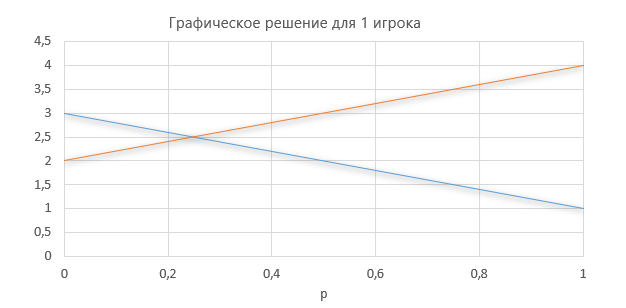
\includegraphics[scale=0.6]{images/1.png}
  Рис. 1: Графическое решение для оптимального решения первого игрока
\end{center}

Рассмотрим диаграмму первого игрока. Синяя линия показывает завимость выигрыша первого игрока от $p$ при условии, что второй игрок придерживается своей первой чистой стратегии, то есть выбирает первый столбец матрицы: $q=(1,0)$. Красная линия - если второй игрок придерживается второй чистой стратегии: $q=(0,1)$.

\textit{Линия минимумов} - нижняя огибающая ломаная, описывающая минимальные (худшие) исходы игры для первого игрока в зависимости от выбора им того или иного значения $p$. На этой линии игрок выбирает \textit{точку максимума}.

Эта точка является точкой пересечения двух прямых. Как же найти эти прямые?

Допустим, что первый игрок использует чистую стратегию $p=(1,0)$, а второй игрок $q=(1,0)$. То есть первая точка будет с абсциссой $p_1=1$ и ординатой, лежащей на пересечении первой строки и первого столбца, то есть $E_1 = 1$. Вторая точка будет иметь абсциссу $p_2=0$ (вторая чистая стратегия первого игрока) и ординату (размер выигрыша) на пересечении второй строки и первого столбца $E_2 = 3$.

Находим уравнение прямой по двум точкам:
$$\frac{p-p_1}{p_2-p_1} = \frac{E-E_1}{E_2-E_1}$$
$$E = 3 - 2p$$

Второе уравнение находим аналогично и получаем, что:
$$E = 2p + 2$$

В точке пересечения найдем точку максимума - оптимальную стратегию среди минимумов для первого игрока:
$$3-2p = 2p+2 \Rightarrow p^* = \frac{1}{4} = 0.25$$

Давайте проверим данную формулу по аналитическому решению, полученному ранее:
$$p^{*} = \frac {a_{22}-a_{21}}{C} = \frac{-1}{-4} = 0.25$$

Мы нашли верно с помощью графического метода оптимальную стратегию для первого игрока. Найдем цену игрока при оптимальной стратегии первого игрока:
$$E = \frac{\Delta}{C} \equiv 3 - 2 \cdot 0.25 = 2.5$$

Для второго игрока строится абсолютная идентичная диаграмма. На данной диаграмме показывается зависимость выигрыша первого игрока (проигрыша второго игрока) от $q$ при условии, что первый игрок придерживается первой стратегии, а именно выбирает первую строку.

\begin{center}
  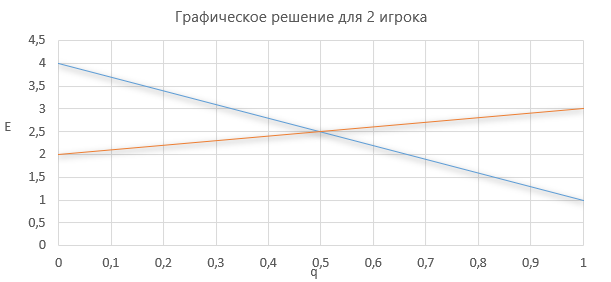
\includegraphics[scale=0.6]{images/2.png}
  Рис. 2: Графическое решение для оптимального решения второго игрока
\end{center}

Выбирается точка минимума - минимума среди максимумов. Эта точка является точкой пересечения двух прямых и является ценой игры. Как искать их мы уже поняли!

Линии на диаграммах разные и пересекаются они в разных точках. Абсциссы этих точек различны. Однако ординаты этих точек равны, ординаты определяют на этих двух диаграммах одну и ту же величину - \textit{размер выигрыша первого игрока}.

Решение приведено в файле:
$$\textsc{2. решение антагонистической игры 2x2.xlsx}$$

\newpage
\subsection{Доминирование стратегий. Теорема об активных стратегиях}

Если платежная матрица имеет седловую точку, то решение игры существует в \textit{чистых стратегиях}, которые определяются седловой точкой матрицы.

Предположим, что седловой точки в платежной матрице нет. Тогда матричную игру следует решать в смешанных стратегиях. Введем следующие определения.

\begin{definition}
  Строка $i$ \textbf{доминирует} строку $k$, если $a_{ij} \geq a_{kj}$ для всех $j = 1,2,\ldots,n$ и существует такой столбец $d$, для которого $a_{id} > a_{kd}$
\end{definition}

Действительно, первый игрок не использует $k$-ую стратегию, так как его выигрыш при $i$-й стратегии не меньше, чем при $j$-й стратегии, вне зависимости от того, как играет второй игрок.
\begin{definition}
  Столбец $j$ \textbf{доминирует} столбец $k$, если $a_{ij} \leq a_{ik}, i = 1,2,\ldots,m$ и существует такая строка $d$, что $a_{dj} < a_{dk}$
\end{definition}

Второй игрок не использует $k$-ую стратегию, так как его проигрыш(равный выигрышу первого игрока) при $j$-ой стратегии не больше, чем при $k$-ой стратегии вне зависимости от того, как играет первый игрок.

\begin{definition}
  Строка, которую доминирует какая-то другая строка, называется \textbf{доминируемой}.
\end{definition}

Если для одного из игроков существует строго доминирующая стратегия, он будет ее использовать в любом из равновесий Нэша в игре. Если все игроки имеют строго доминирующие стратегии, то игра имеет единственное равновесиве Нэша.

\begin{center}
  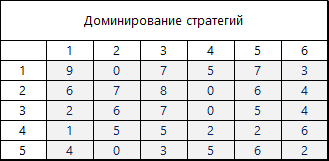
\includegraphics[scale=0.5]{images/3.png}

  Рис. 3: Доминирование строк и столбцов
\end{center}

В данном случае $2$-ая строка доминирует над $3$-ей строкой, а $1$-ая на $5$-ой. $2$-ой столбец доминирует $3$-ий столбец, а $4$-ый - $5$-ый.

Последовательное исключение доминируемых стратегий - часто используемая тезнология решения или упрощения игр. Она основана на предположении о том, что в процессе игры стороны не будут использовать \textit{доминируемы стратегии}, в связи с чем их можно не рассматривать при дальнейшем решении (вероятность выбора данной строки будет равна нулю) и приписать им нулевые вероятности. На цене игры это никак не скажется, а размерность матрицы игры понизится. С этого и нужно начинать решение игры.

Если платежная матрица содержит несколько одинаковых строк (столбцов), то из них мы оставляем лишь одну строку, а остальные отбрасываем. Такой частный случай доминирования является \textbf{дублированием стратегий}.

Однако, исключение этих стратегий из рассмотрения приводит к сужению множества возможных ситуаций, в результате чего могут возникнуть новые доминируемые стратегии, которые в исходной игре не доминировались.

В некоторых играх, в зависимости от последовательности удаления слабо доминируемых стратегий, процесс итеративного исключения может сходиться к различным равновесиям Нэша.

Решение приведено в файле:
$$\textsc{3. доминирование строк и столбцов.xlsx}$$

\subsubsection{Теорема об активных стратегиях}

\begin{definition}
  Чистая стратегия $i$ называется \textbf{активной стратегией}, если она используется в некоторой оптимальной смешанной стратегии с положительной, ненулевой вероятностью.
\end{definition}

\begin{theorem}
  Теорема об активных стратегиях (доказательство ?)

  Если один из игроков придерживается своей оптимальной смешанной стратегии, то выигрыш остается неизменным и равным цене игры $E$, если второй игрок не выходит за пределы своих активных стратегий, причем количество активных стратегий равно: $L = \min(m,n)$.
\end{theorem}

Эта теорема имеет большое практическое значение - она дает конкретные модели нахождения оптимальных стратегий при отсутствии седловой точки.

\subsubsection{Решение игр 2xn графическим методом}

При решении задачи $2 \times n$ графическим методом алгоритм действий следующий:

\begin{enumerate}
  \item С самого начала нам дана матрица, где у первого игрока есть $2$ возможные стратегии, а у второго игрока $n$ возможных стратегий. Данную матрицу мы проверяем на наличие седловой точки. 

  Сначала мы находим \textit{максимин} первого игрока - тот минимальный выигрыш, который получит первый игрок, если выберет строку. Максимин также является \textit{нижней ценой игры}. Затем мы находим \textit{минимакс} - гарантированный проигрыш второго игрока - \textit{верхняя цена игры}. 

  Если данные значения совпали, то, следовательно, нижняя цена игры совпала с верхней, цена равна минимаксу (максимину). Следовательно, есть седловая точка и решение, как известно, существует в \textit{чистых стратегиях}, которое мы и находим.

  \item Если седловая точка отсутствует, то будем искать решение в смешанных стратегиях. Построим некую огибающую семейства графиков - \textbf{ломаная, описывающая минимальны исходы игры первого игрока в зависимости от выбора им того или иного значения $p$} и по ней определим искомую точку и соответствующая ей вероятность. 

  Минимальные исходы первого игрока ищутся через математическое ожидание выигрыша. 
  $$E = PAQ^T$$
  где $P=(p,1-p) \quad 1 \times 2$, $A$ - матрица игры $2 \times n$, а $$Q = (q_1,\ldots,q_n) \quad 1 \times n$$ - вектор смешанных стратегий второго игрока. 

  Если мы посчитаем для каждой чистой стратегии (всего $n$ ) второго игрока математические ожидания выигрыша первого игрока и потом возьмем минимум среди всех $n$ математических ожиданий, то таким образом на каждом шаге вероятности $p$ мы будем вычислять точки \textit{линии огибающую семейство графиков}.

  На этой линии выберем точку максимума. Точность будет зависеть от шага дробления вероятности.
  \item По теореме об активных стратегиях, найдутся $2$ активные стратегии у второго игрока и мы выделяем из исходной матрицы матрицу $2 \times 2$, состоящую из стратегий первого игрока и активных стратегий второго
  \item После этого решается антагонистическая игра $2 \times 2$ теми методами, которые были рассмотрены ранее: проверяется на наличие седловой точки, вычисляется цены игры по формуле $E=\frac{\Delta}{C}$.
  \item Строятся уточненные ответы, в которых на месте неактивных стратегий второго игрока будут нули, а на месте активных - распределение вероятностей - смешанные стратегии первого и второго игрока.
\end{enumerate}

\subsubsection{Решение игр mx2 графическим методом}

Суть метода абсолютно тот же самый и, чтобы было удобно, мы транспонируем матрицу $m\times 2$ и получаем матрицу $2 \times m$, где в качестве строк выступают смешанные стратегии второго игрока, а в качестве столбцов - первого.

Различие при поиска максиминов будет в том, что так как в строках находится гарантированный проигрыш второго игрока, то мы будем искать по строкам максимум и потом найдем среди них минимум - \textit{по строкам - максимин}, а по столбцам, соответственно, минимакс.

Мы строим верхнюю огибающую линию - \textbf{ломаную, описывающую максимальные проигрыши второго игрока}. Поэтому на данной ломаной выберем \textit{точку минимума}.

После этого выбираем $2$ активные стратегии среди $p$ и строим матрицу $2 \times 2$, которая и даст нам решение.

Реализация графического метода для данных двух случаев приведена в этом файле:
$$\textsc{4. 2xn, mx2, антагонистические игры, графичекое решение.xlsx}$$

\newpage
\subsection{Существование решения игры в смешанных стратегиях}

Пусть дана антагонистическая игра с матрицей $A$ размерности $m \times n$
$$A = \begin{bmatrix}
  a_{11} & a_{12} & \ldots & a_{1n} \\
  a_{21} & a_{22} & \ldots & a_{2n} \\
  \ldots & \ldots & \ldots & \ldots \\
  a_{m1} & a_{m2} & \ldots & a_{mn}
\end{bmatrix}$$

Решение смешанного расширения игры является седловая точка матрицы в смешанных стратегиях, то есть такие два стохастических вектора, вектор $P^* = (p_1^*,\ldots,p_m^*)$ и вектор $Q^* = (q_1^8,q_2^*,\ldots,q_m^*)$, что для любых стохастических векторов $P$ и $Q$ соответствующей размерности выполнены равенства:
$$PAQ^{*T} \leq P^*AQ^{*T} \leq P^*AQ^T \eqno (1)$$

\begin{theorem}
  Основная теорема Нэша

  В любой матричной антагонистической игре существует такая пара смешанных стратегий $(P^*,Q^*)$, что:
  $$PAQ^{*T} \leq P^*AQ^{*T} \leq P^*AQ^T \eqno $$
  $$E(p,q^*) \leq E(p^*,q^*) \leq E(p^*,q)$$

  И цена игры равна $E(p^*,q^*)$ и можно указать \textit{алгоритм построения этого решения}.
\end{theorem}

\begin{proof}
Попытаемся доказать это утверждение. Начнем с леммы

\begin{definition}
  \textit{Афинное преобразование} - отображение плоскости или пространства на себя, при котором параллельные прямые переходят в параллельные, пересекающиеся - в пересекающиеся, скрещивающеся - в скрещивающиеся.
\end{definition}

Рассмотрим матрицу $B$, связанную с матрицей $A$ соотношением:
$$B = c \times A + D \eqno (2)$$
где $c>0$ константа, а $D$ - матрица $m \times n$, все элементы которой одинаковы и обозначим их посредством $d$. Такое преобразвание матрицы $A$ в $B$ относится к классу афинных преобразований.

\begin{lemma}
  Лемма об афинном преобразовании матрицы игры

  Всякая седловая точка матрицы $A$ является седловой точкой матрицы $B$
\end{lemma}
\begin{proof}
  Пусть пара $(P^*,Q^*)$ - седловая точка матрицы $A$. Докажем, что она является седловой для матрицы $B$, то есть:
  $$PBQ^{*T} \leq P^*BQ^{*T} \leq P^*BQ^T \eqno (3)$$

  Для этого домножим все части неравенства на $c>0$ и добавим ко всем частям константу $d$. Знаки неравенств сохранятся:
  $$cPAQ^{*T} + d \leq cP^*AQ^{*T} + d \leq cP^*AQ^T + d \eqno (3)$$
  $$PcAQ^{*T} + d \leq P^*cAQ^{*T} + d \leq P^*cAQ^T + d \eqno (4)$$

  Заметим, что для любых стохастических вектором $P$ и $Q$ выполнятся равенства:
  $$PDQ^T = dPJ_{m,n}Q^T = (\sum\limits_{i=1}^m p_i,\ldots,\sum\limits_{i=1}^m p_i)Q^T = J_{1,n}Q^T = d \eqno (6)$$
  где $J_{m,n}$ - единичная матрица размера $m \times n$.

  Таким образом:
  $$PcAQ^{*T} + PDQ^{*T}  \leq P^*cAQ^{*T} + P^*DQ^{*T} \leq P^*cAQ^T + P^*DQ^{T} \eqno (7)$$

  В каждой части неравенства выносим за скобки первый множитель и последний (выносим право) и с помощью равенства $(2)$получаем неравенство, которое нам и нужно было доказать:
  $$PBQ^{*T} \leq P^*BQ^{*T} \leq P^*BQ^T \eqno (3)$$
\end{proof}

\textbf{Замечание:} аналогично доказывается, что всякая седловая точка матрицы $B$ является седловой точкой матрицы $A$.

\textbf{Замечание:} если $H$ и $H'$ - цены игр матриц $A$ и $B$ соответственно, то:
$$H' = cH + d$$

Разобрать доказательство из файла решение антагонистических игр в смешанных стратегиях

\subsubsection{Сведение игры к паре сопряженных задач линейного программирования}

\textbf{Сведение решения игры к решению ЗЛП для первого игрока}

Матрица $A$ может содержать как положительные, так и отрицательные элементы. Возьмем такую достаточно большую константу $d$, что все элементы матрицы $B$:
$$B = A + D$$
были положительными. Для этого можно взять $d = \min \{a_{ij}\} + 1$, например. Матрица $B$ имеет вид:
$$B = \begin{bmatrix}
  b_{11} & b_{12} & \ldots & b_{1n} \\
  b_{21} & b_{22} & \ldots & b_{2n} \\
  \ldots & \ldots & \ldots & \ldots \\
  b_{m1} & b_{m2} & \ldots & b_{mn}
\end{bmatrix}$$

У данной матрицы $B$ седловая точка находится на той же позиции, что у матрицы $A$ (по прошлой лемме). И мы будем искать седловую точку матрицы $B$.

Пусть первый игрок выбрал некоторую смешанную стратегию $P = (p_1,\ldots,p_m)$. Если второй игрок выбрал свою $n$-ую чистую стратегию, то первый получил выигрыш: $b_{1n}p_1+b_{2n}p_2 + \ldots + b_{mn}p_m$.

Первый игрок хочет получить максимально возможный гарантированный выигрыш. Он ограничивает снизу все эти выражения величиной $v$, чтобы \textit{каждый выигрыш первого игрока был не меньше этой величины}, которую стремится максимизировать. Возникает следующая задача линейного программирования:
$$\begin{cases}
  b_{11}p_1+b_{21}p_2 + \ldots + b_{m1}p_m \geq v \\
  b_{12}p_1+b_{22}p_2 + \ldots + b_{m2}p_m \geq v \\
  \ldots \ldots \ldots \ldots \ldots\ldots \ldots \ldots \ldots \ldots  \\
  b_{1n}p_1+b_{2n}p_2 + \ldots + b_{mn}p_m \geq v
\end{cases}$$
$$v \to \max \qquad \sum\limits_{i=1}^m p_i = 1 \qquad p_i  \geq 0, i = 1,\ldots,m$$

Можно переписать задачу, учитывая, что все элементы матрицы $B$ положительные, то можно выбрать величину $v$ в качестве наименьшего значения матрицы $B$ и поделить блоки неравенств на $v$.
$$x_i = \frac{p_i}{v} \qquad \sum\limits_{i=1}^m x_i = \frac{1}{v}$$
и тогда максимизация $v$ равносильна минимазации выражения $\sum\limits_{i=1}^m x_i$ и сформулированная ЗЛП первого игрока можно преобразовать к виду:
$$\begin{cases}
  b_{11}x_1+b_{21}x_2 + \ldots + b_{m1}x_m \geq 1 \\
  b_{12}x_1+b_{22}x_2 + \ldots + b_{m2}x_m \geq 1 \\
  \ldots \ldots \ldots \ldots \ldots\ldots \ldots \ldots \ldots \ldots  \\
  b_{1n}x_1+b_{2n}x_2 + \ldots + b_{mn}x_m \geq 1
\end{cases}$$
$$\sum\limits_{i=1}^m x_i \to \min, x_i \geq 0, i = 1,\ldots,m$$
где матрица системы ограничений есть трансонированная матрица $B$.

Решив данную задачу линейного программирования, получим ее оптимальный план: набор значений $x_i$. Откуда найдем:
$$v = \frac{1}{\sum\limits_{i=1}^m x_i}$$
$$p_i = x_i \cdot v = \frac{x_i}{\sum\limits_{i=1}^m x_i}$$
$v$ - максимальный выигрыш первого игрока для матрицы $B$

Вероятности $p_i$, согласно лемме, годятся и для исходной игры с матрицей $A$. Размер выигрыша $v$ связан с матрицей $B$. Для матрицы $A$, согласно второму замечанию после леммы предыдущего параграфа при $c=1$ выигрыш первого игрока в игре с матрицей $A$:
$$V = v - d$$

\textbf{Сведение решения игры к решению ЗЛП для второго игрока}

Матрица $A$ может содержать как положительные, так и отрицательные элементы. Возьмем такую достаточно большую константу $d$, что все элементы матрицы $B$:
$$B = A + D$$
были положительными. Для этого можно взять $d = \min \{a_{ij}\} + 1$, например. Матрица $B$ имеет вид:
$$B = \begin{bmatrix}
  b_{11} & b_{12} & \ldots & b_{1n} \\
  b_{21} & b_{22} & \ldots & b_{2n} \\
  \ldots & \ldots & \ldots & \ldots \\
  b_{m1} & b_{m2} & \ldots & b_{mn}
\end{bmatrix}$$

У данной матрицы $B$ седловая точка находится на той же позиции, что у матрицы $A$ (по прошлой лемме). И мы будем искать седловую точку матрицы $B$.

Пусть второй игрок выбрал некоторую смешанную стратегию $Q = (q_1,\ldots,q_n)$. Если второй игрок выбрал свою $m$-ую чистую стратегию, то второй получил соответственно проигрыш (выигрыш первого игрока): $b_{m1}q_1+b_{m2}q_2 + \ldots + b_{mn}q_n$.

Второй игрок хочет получить минимально возможный гарантированный проигрыш. Он ограничивает сверху все эти выражения величиной $v$, чтобы \textit{каждый проигрыш второго игрока был не больше этой величины}, которую стремится минимизировать. Возникает следующая задача линейного программирования:
$$\begin{cases}
  b_{11}q_1+b_{12}q_2 + \ldots + b_{1n}q_n \leq v \\
  b_{21}q_1+b_{22}q_2 + \ldots + b_{2n}q_n \leq v \\
  \ldots \ldots \ldots \ldots \ldots\ldots \ldots \ldots \ldots \ldots  \\
  b_{m1}q_1+b_{m2}q_2 + \ldots + b_{mn}q_n \leq v
\end{cases}$$
$$v \to \min \qquad \sum\limits_{j=1}^n q_j = 1 \qquad q_j  \geq 0, j = 1,\ldots,n$$

Можно переписать задачу, учитывая, что все элементы матрицы $B$ положительные, то можно выбрать величину $v$ в качестве максимального значения матрицы $B$ и поделить блоки неравенств на $v$.
$$y_j = \frac{q_j}{v} \qquad \sum\limits_{j=1}^n y_j = \frac{1}{v}$$
и тогда минимизация $v$ равносильна максимизации выражения $\sum\limits_{j=1}^n y_j$ и сформулированная ЗЛП второго игрока можно преобразовать к виду:
$$\begin{cases}
  b_{11}y_1+b_{12}y_2 + \ldots + b_{1n}y_n \leq 1 \\
  b_{21}y_1+b_{22}y_2 + \ldots + b_{2n}y_n \leq 1 \\
  \ldots \ldots \ldots \ldots \ldots\ldots \ldots \ldots \ldots \ldots  \\
  b_{m1}y_1+b_{m2}y_2 + \ldots + b_{mn}y_n \leq 1
\end{cases}$$
$$\sum\limits_{j=1}^n y_j \to \max, y_j \geq 0, j = 1,\ldots,n$$
где матрица системы ограничений есть матрица $B$.

Решив данную задачу линейного программирования (если решение существует), получим ее оптимальный план: набор значений $y_j$. Откуда найдем:
$$v = \frac{1}{\sum\limits_{j=1}^n y_j}$$
$$q_j = y_j \cdot v = \frac{y_j}{\sum\limits_{j=1}^n y_j}$$
$v$ - минимальный проигрыш второго игрока(максимальный выигрыш первого игрока для матрицы) $B$.

Вероятности $q_j$, согласно лемме, годятся и для исходной игры с матрицей $A$. Размер выигрыша $v$ связан с матрицей $B$. Для матрицы $A$, согласно второму замечанию после леммы предыдущего параграфа при $c=1$ выигрыш первого игрока в игре с матрицей $A$:
$$V = v - d$$
$V$ - выигрыш первого игрока в игре с матрицей $A$ (проигрыш второго игрока).

\textbf{Финальный шаг доказательства теоремы о существовании решения игры в смешанных стратегиях}

Рассмотрим ЗЛП для первого игрока
$$\begin{cases}
  b_{11}x_1+b_{21}x_2 + \ldots + b_{m1}x_m \geq 1 \\
  b_{12}x_1+b_{22}x_2 + \ldots + b_{m2}x_m \geq 1 \\
  \ldots \ldots \ldots \ldots \ldots\ldots \ldots \ldots \ldots \ldots  \\
  b_{1n}x_1+b_{2n}x_2 + \ldots + b_{mn}x_m \geq 1
\end{cases}$$
$$\sum\limits_{i=1}^m x_i \to \min, x_i \geq 0, i = 1,\ldots,m$$

и запишем ее в другом виде:
$$\sum\limits_{i=1}^m c_i \cdot x_i \to \min,\quad  x_i \geq 0, c_i=1, i =1,\ldots,m$$
$$\sum\limits_{i=1}^m b_{ij} \cdot x_i \geq a_j, a_j = 1, j = 1 \ldots n$$

Теперь попытаемся по данной задаче построить двойственную задачу по правилам построения:

\begin{enumerate}
  \item коэффициенты $a_j$ - коэффициенты целевой функции двойственной задачи при переменных $y_j$
  \item каждое ограничение, коих $n$, порождает переменную $y_j$
  \item $x_i$ являются $i$-м ограничением двойственной задачи
  \item $c_i$ - константы в правых частях $i$-х ограничений двойственной зачачи
  \item целевая функция двойственной задачи стремиться теперь не к минимуму, а к максимуму
  \item знаки ограничений меняются на противоположные, то есть на $\leq$. 
\end{enumerate}

Если по данным правилам мы построим двойственную задачу, то увидим, что она совпадает с той задачей, что мы построили для второго игрока:
$$\begin{cases}
  b_{11}y_1+b_{12}y_2 + \ldots + b_{1n}y_n \leq 1 \\
  b_{21}y_1+b_{22}y_2 + \ldots + b_{2n}y_n \leq 1 \\
  \ldots \ldots \ldots \ldots \ldots\ldots \ldots \ldots \ldots \ldots  \\
  b_{m1}y_1+b_{m2}y_2 + \ldots + b_{mn}y_n \leq 1
\end{cases}$$
$$\sum\limits_{j=1}^n y_j \to \max, y_j \geq 0, j = 1,\ldots,n$$

Запишем в другом виде для наглядности:
$$\sum\limits_{j=1}^n a_j \cdot y_j \to \max,\qquad  y_j \geq 0, a_j = 1 j = 1,\ldots,n$$
$$\sum\limits_{j=1}^n b_{ij} \cdot y_j \leq c_i, c_i = 1, i = 1 \ldots m$$
Следовательно, данные задачи взаимно двойственны.

\begin{theorem}
  Критерий оптимальности Канторовича

  Если на допустимых планах значения их целевых функция совпадают, то планы являются оптимальными.
\end{theorem}

\begin{theorem}
  А для существование оптимальных решений как прямой, так и двойственной задачи, необходимо и достаточно существование какого-либо допустимого плана для каждой из них.
\end{theorem}

Для данных планов решение существует, например, нулевое для двойственной задачи.

\begin{theorem}
  Если прямая (двойственная) задача имеет оптимальное решение, то и двойственная (прямая) задача имеет оптимальное решение
\end{theorem}

Следовательно, по данным теоремам, задачи явлются взаимо двойственны и мы нашли допустимый план для каждой из задач, следовательно у этих задач есть оптимальное решение и оно одинаковое, как и должно быть в антагонистической матрице (выигрыш первого игрока равен проигрышу второго). На этом доказательство основной теоремы антагонистических игр Нэша заканчивается.
\end{proof}

Получи оптимальные планы $x_i$ и $y_j$ мы по формулам выведенным получим оптимальные смешанные стратегии игроков и размер выигрыша первого игрока (проигрыша второго).

В основе решения ЗЛП лежит симплекс-метод. Получить решение можно, например, через Excel, воспользовавшись процедурой "Поиск решения".

Заметим, что Отчет об устойчивости, сопровождающий такое решение задачи, содержит \textit{теневые цены} – компоненты
оптимального плана двойственной задачи (для получения такого отчета следует в качестве
метода решения выбрать именно симплекс-метод). Таким образом, решая одну из задач, мы
попутно получаем решение и другой.

Реализация линейного программирования выполнена в файле:
$$\textsc{5. линейное программирование.xlsx}$$

\subsubsection{Алгоритм решения матричных игр}

Соответственно алгоритм решения матричных игр может быть представлен следующий:

\begin{itemize}
  \item Мы сначала отбрасываем доминируемые строки, которые будут входит в ответ с нулевой вероятностью, уменьшая матрицу
  \item Затем сводим матрицу к задаче линейного программирования способом, описанным выше и находим ее цену игры
\end{itemize}

\subsubsection{Имитационная проверка решения задачи линейного программирования}

Допустим, что нами был реализован способ решения матричной игры с помощью сведению к линейному программированию. Посмотрим, как это было реализовано в Excel.

\begin{center}
  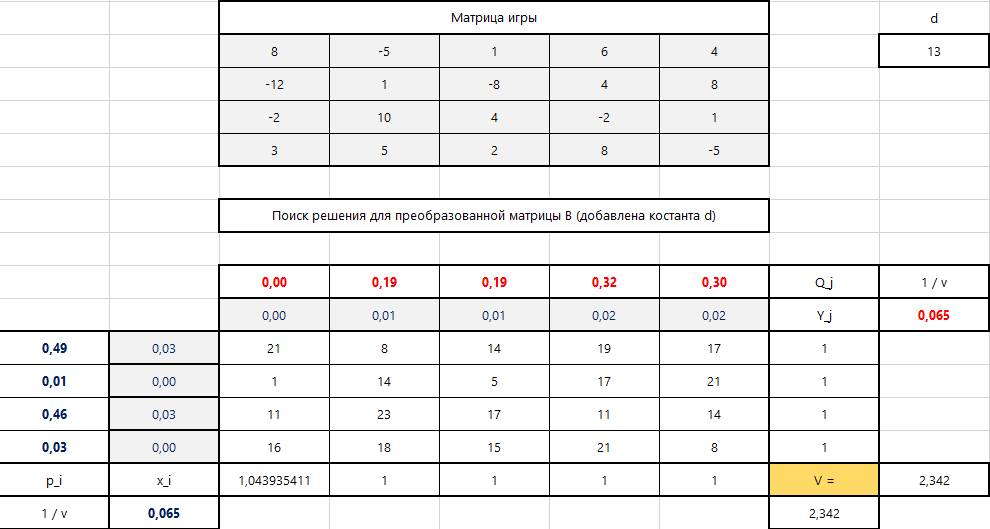
\includegraphics[scale=0.37]{images/4.png}
  Рис. 4: Решение матричной игры с помощью линейного программирования
\end{center}

Постараемся имитационно проверить решение данной игры.

\begin{center}
  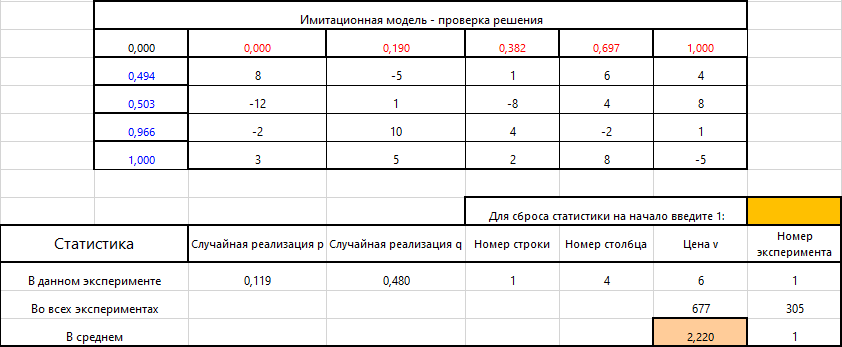
\includegraphics[scale=0.37]{images/5.png}

  Рис. 5: Имитационное моделирование, проверка решения
\end{center}

По смешанным стратегиям $p,q$, которое было получено при решении задачи линейного программирования, можно построить функцию распределения вероятности выбора строки (столбца) для каждого игрока. После этого с помощью функции \textsc{СЛЧИС()} будем на каждом шаге проделывать реализацию случайной величины и смотреть, какая чистая стратегия каждого игрока использовалась в каждой конкректной реализации. Пересечением выбора чистых стратегий является элемент матрицы, являющися ценой выигрыша первого игрока (проигрыша второго).

Будем искать среднее значение на протяжение всего имитационного процесса и в конечном счете получим значение, близкое к реальной цене игры. Но скорость сходимости данного имитационного процесса очень маленькая, поэтому был придуман следующий итерационный метод.

\newpage
\subsection{Метод Брауна}

Пусть игра матрицы задана матрицей $A$ размерности $m \times n$. 

\begin{definition}
  Каждое разыгрывание игры в \textit{чистых стратегиях} называется \textbf{партией}.
\end{definition}

Метод Брауна - это итеративная процедура построения \textit{последовательности пар смешанных стратегий игроков}, \textbf{сходящейся к решению матричной игры}.

В $1$-ой партии оба игрока выбирают произвольную чистую стратегию. Пусть сыграно $k$ партий, причем выбор стратегии в каждой партии запоминается. В $(k+1)$-ой партии каждый игрок выбирает ту чистую стратегию, которая максимизирует его ожидаемый выигрыш, если противник играет в соответствии с эмперическим вероятностным распределением, сформировавшимся за $k$ партий. На каждом шаге оценивается интервал для цены игры и, если он достаточно мал, то процесс останавливается. Полученные при этом вероятностые распределения определяют смешанные стратегии игроков.

Пусть первые $k$ партий первый игрок использовал $i$-ую статегию $\xi_i^k$ раз $i=1,\ldots,m$, а второй игрок свою $j$-ую стратегию $\eta_j^k$ раз $j=1,\ldots,n$. Тогда первый игрок полагает, что его противник будет следовать смешанной стратегии:
$$y^k = \left(\frac{\eta_1^k}{k},\frac{\eta_2^k}{k}, \ldots,\frac{\eta_1^n}{k}\right)$$
а второй игрок, в свою очередь, полагает, что первый последует согласно смешанной стратегии:
$$x^k = \left(\frac{\xi_1^k}{k},\frac{\xi_2^k}{k}, \ldots,\frac{\xi_1^m}{k}\right)$$


Значит при следующем разбиении на $(k+1)$-ой партии они сыграют так:
$$\text{Первый игрок выбирает:} \qquad i_{k+1}:\sum\limits_{j}a_{i_{k+1},j}\eta_j^k = \underset{i}{\max}\sum\limits_j a_{ij}\eta_j^k = \bar{v}^k$$
то есть выбирает максимальный выигрыш для себя среди всех строк, умноженных на вероятность выбора стратегии вторым игроком, расчитанную по предыдущим $k$ играм.
$$\text{А второй игрок выбирает:} \qquad j_{k+1}:\sum\limits_{i}a_{i,j_{k+1}}\xi_i^k = \underset{j}{\min} \sum\limits_i a_{ij}\xi_i^k = \underline{v}^k$$
то есть выбирает \textit{минимальный проигрыш для себя} по столбцам, умноженным на вероятность выбра стратегии первым игроком, расчитанную по предыдущим $k$ играм.

Через $\bar{v}^k$ и $\underline{v}^k$ обозначены $k$-ые приближения верхней и нижней игры соответственно. Легко видеть, что:
$$\frac{\bar{v}^k}{k} = \underset{i}{\max}\sum\limits_j a_{ij}\frac{\eta_j^k}{k} = \sum\limits_{j}a_{i_{k+1},j}\frac{\eta_j^k}{k} $$
$$\frac{\overline{v}^k}{k} = \underset{j}{\min}\sum\limits_i a_{ij}\frac{\xi_i^k}{k} = \sum\limits_{i}a_{i,j_{k+1}}\frac{\xi_i^k}{k} $$

По определинию цены игры - если нижняя и верхняя цена совпадает, то есть если матрица сожержит элемент, которя является минимальным в своей строке и одновременно максимальным в своем столбце. Нижняя цена - максимин, верхняя цена - минимакс, максимин меньше минимакса, следовательно:
$$\underset{k}{\max} \frac{\overline{v}^k}{k} \leq v \leq \underset{k}{\min} \frac{\overline{v}^k}{k}$$
где $v$ - реальная цена игры.

Итеративнй процесс сходится к истинному значению игры, то есть:
$$\lim\limits_{k \to\infty} \underset{k}{\max} \frac{\overline{v}^k}{k} = \lim\limits_{k \to\infty} \underset{k}{\min} \frac{\overline{v}^k}{k} = v$$

Итерационный процесс метода Брауна не является монотонным, кроме того, скорость сходимости метода быстро уменьшается с ростом размерности матрицы игры. Однако он обладает одним неиспоримым преимуществом, которое заключается в простоте программирования метода.

В конечном счете, при сходимости итерационным методом Брауна, то есть при равенстве итерационной цены игры теоретической, в качестве ответа будет вероятности стратегий каждого игрока, то есть смешанные стратегии, которые должны совпасть с точным ответом.

В качестве цены игры, как это и логично и понятно, вычисляется математическое ожидание выигрыша первого игрока:
$$E = PAQ^T$$

\subsubsection{Реализация метода Брауна средствами Excel}

Реализация итерационного метода Брауна представлена в файле:
$$\textsc{6. метода брауна.xlsx}$$

\newpage
\subsection{Игра Блотто}

Полковник Блотто – мифический персонаж, созданный фантазией одного из авторов. У полковника Блотто $n$ солдат, а у его противника $m$ солдат. Полковнику нужно защитить $k$ участков фронта, противник пытается прорваться на этих участках. Все солдаты предполагаются одинаковыми, их можно рассматривать как единицы однородного ресурса.

Полковник и его противник по своему усмотрению расставляют солдат по участкам, не зная действий противоположной стороны. На каждом участке побеждает та сторона, у которой \textbf{больше солдат}. \textit{Выигрыш стороны} определяется \textbf{количеством участков}, на которых одержана победа (выигрыш может оказаться и отрицательной величиной).

\begin{definition}
  \textbf{Игра полковника Блотто} – модельное представление задачи о правильном распределении ограниченного ресурса в условиях активного противодействия. Это антагонистическая игра. Рассмотрим конкретный вариант игры с тремя участками и тремя солдатами с каждой стороны.
\end{definition}

Игру можно представить в матричной форме. Расстановки полковника указаны в начале строк, расстановки противника – в начале столбцов. Например, $300$ означает, что на первом участке стоят $3$ солдата, на остальных по $0$. В ячейках указана величина выигрыша
полковника в соответствующей ситуации. Выигрыш противника – это та же величина, но с обратным знаком; она подразумевается, но в матрице в явном виде не указывается.

\begin{center}
  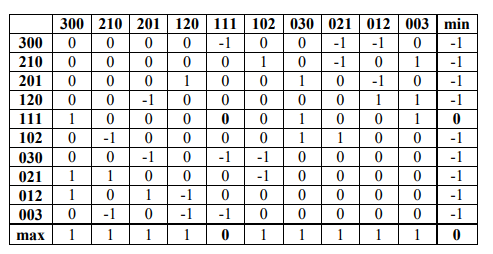
\includegraphics[scale=0.6]{images/12.png}

  \textbf{Матрица игры Блотто}
\end{center}

Полковник проводит анализ матрицы (как и его противник). Для каждой своей стратегии – строки матрицы он рассматривает худший исход. Этот худший исход характеризуется минимальной величиной выигрыша в данной строке. Все минимумы он выписывает справа от матрицы. Из всех худших исходов он выбирает лучший – максимум среди минимумов. Такая величина называется \textit{максимином}. Это $0$ в средней строке.

Аналогичный анализ матрицы проводит его противник. Его стратегии – это столбцы матрицы, а худший исход характеризуется максимумом в столбце. Он выписывает их под матрицей. Как и Блотто, он из худших вариантов выбирает лучший. Это минимум среди
максимумов – минимакс. таким минимаксом является $0$ в среднем столбце.

Таким образом оба игрока выбирают стратегии $111$, расставляя по одному солдату на
участок. При этом оба игрока защищают все участки и не могут прорваться. Эта ситуация является \textit{седловой точкой матрицы}, она соответствует \textit{равновесию по Нэшу}. 

\newpage
\subsection{Игра инспекция, формулы решения}

\begin{definition}
  \textit{Игра Инспекция} - это многоходовая антагонистическая игра, описывающая взаимодействие двух лиц во времени, представляющая важную и распространенную модель поведения.
\end{definition}

На каждом ходу \textbf{нарушитель (игрок 1)} может нарушить некое правило, а \textbf{инспектор (игрок 2)} может проверить наличие нарушения. Если это происходит в одном периоде, то нарушение выявляется, если в разных, то нет.

Модификации игры:

\begin{enumerate}
  \item Во-первых, величина штрафа и величина выигрыша в реальности могут существенно различаться. Выигрыш обозначм за $1$, а штраф за $-M$.
  \item Возможны варианты игры: когда результыт очередного шага становятся известны обоим игрокам, или же когда они не известны им до конца игры. 
  \item В-третьих, мы проанализируем не только вариант, когда игроки до конца игры могут действовать или бездействовать, но и вариант, когда они обязаны действовать
\end{enumerate}

Игра продолжается $N$ периодов времени, по результатам игры первый игрок получает выигрыш величины $V_N$.

\subsubsection{Игра инспекция с обязательной активностью игроков}

\textit{Обязательная активность} - каждый игрок должен проявить активность в каком-то периоде времени. Мы покажем, что информация о результатах не меняет стратегии игроков - рекурсивное и матричное представление дают одни и те же результаты.

\textbf{Рекурсивное представление игры}

У каждого игрока есть $N$ статегий, соответствующих выбору того или иного периода времени для активного действия.

\textit{Действие игрока} - нарушение правил для одного игрока либо инспеция нарушения для второго.

При $N=1$ матрица \textsc{Нарушителя} $A_1$ имеет размерность $1 \times 1$ (так как нарушитель обязан действовать, а инспектор - проверить). Следовательно, второй игрок обязательно поймает нарушителя и ему будет выписан штраф $-M$.
$$A_1 = - M_1$$

При этом выигрыш первого игрока составит $V_1 = -M$.

При произвольном $N>1$ матрица \textsc{Нарушителя} $A_N$ имеет вид:
$$A_N = \begin{bmatrix}
  -M & 1 \\ 1 & V_{N-1}
\end{bmatrix}$$

Это матрица действия игроков в периоде $N$. Строки соответствуют действиям \textsc{Нарушителя}, столбцы - \textsc{Инспектора}. 

Первая строка и первый столбец - активное поведение игроков (нарушение для \textsc{Нарушителя} и проверка для \textsc{инспектора}).

Вторая строка и второй столбец - пассивное поведение (не нарушение и не проверка соответственно).

Элементы данной матрицы  - это выигрыши \textsc{Нарушителя} по результатам игры в целом (не только этого хода).

\begin{proof}
  Действительно

  \begin{itemize}
    \item элемент $a_{11} = - M$, поскольку если \textsc{Нарушитель} нарушил и инспекция произошла в том же периоде, то нарушение вскрыто и нарушитель платит штраф в размере $-M$
    \item элемент $a_{12} = 1$, так как если \textsc{Нарушитель} нарушил и инспекции не было, то \textsc{Нарушитель} получает выигрыш, равный $1$
    \item $a_{21}=1$, так как если инспекция прошла, а нарушитель не нарушил, то он имеет открытую возможность нарушить на следующем ходу и получить $1$ в качестве выигрыша. Предполагается, что в очередном периоде игрокам известна история предшествующих периодов.
    \item $a_{22} = V_{N-1}$ - оба игрока бездействовали, игра сводится к такой же игре с числом ходов, меньшим на $1$. Игра сводится к такой же игре, но с меньшим числом периодов. Анализ игры имеет рекурсивную форму
  \end{itemize}
\end{proof}

Заметим, что $V_{n-1}<1$, иначе бы $a_{21}=1$ был бы минимумом в строке и максимумом в столбце и \textsc{Нарушитель} бы всегда выигрывал (эта стратегия была бы выгодна ему всегда).

По формуле цены игры с матрицей $2\times 2$ имеем:
$$V_N = \frac{\Delta}{C} = \frac{-MV_{N-1}-1}{-M+V_{N-1}-2} = \frac{MV_{N-1}+1}{M+2-V_{N-1}}$$

Отсюда при $V_1 = -M$:
$$V_2 = \frac{-M^2+1}{2M+2} = \frac{1-M}{2}$$
$$V_3 = \frac{2-M}{3}$$
$$V_4 = \frac{3-M}{4}$$

Формируем гипотезу про формулу для величины $V_N$ и проведем доказательство методом индукции:

\begin{theorem}
  Цена игры инспекции:
  $$V_N = 1 - \frac{M+1}{N}$$
\end{theorem}
\begin{proof}
  База верна. Предположим, что верно наше утверждение. Докажем, что и для $N+1$ тоже будет верно:
  $$V_{N+1} = \frac{MV_{N-1}+1}{M+2-V_{N-1}} = \frac{M\left(1 - \frac{M+1}{N}\right)+1}{M+2-\left(1 - \frac{M+1}{N}\right)} = \frac{N-M}{N+1} = 1 - \frac{M+1}{N+1}$$
  Следовательно, формула доказана по индукции
\end{proof}

Соответственно, цены игры $V_{N-1}$ равна:
$$V_{N-1} = 1 - \frac{M+1}{N-1}$$

Подставим $V_{N-1}$ в исходную матрицу:
$$A_N = \begin{bmatrix}
  -M & 1 \\ 1 & 1 - \frac{M+1}{N-1}
\end{bmatrix}$$

Тогда по формулам, выведенным при решении антагонистических игр $2\times 2$ найдем оптимальные стратегии:
$$p^{*} = \frac {a_{22}-a_{21}}{C}  = \frac{1 - \frac{M+1}{N-1}-1}{-M+1 - \frac{M+1}{N-1}-2} = \frac{1}{N}$$
$$1-p^{*} = \frac{a_{11} - a_{12}}{C}  = 1 - \frac{1}{N} = \frac{N-1}{N}$$

Как видно, вероятности не зависят от величины штрафа $M$. Нарушитель с вероятностью $\frac{1}{N}$ нарушает в первом периоде для $N$-шаговой игры. Матрица симметрична и вероятности для инспектора такие же.
$$q^{*} = \frac {a_{22}-a_{12}}{C} = \frac{1 - \frac{M+1}{N-1}-1}{-M+1 - \frac{M+1}{N-1}-2} = \frac{1}{N}$$
$$1-q^{*} = \frac{a_{11} - a_{21}}{C}  = 1 - \frac{1}{N} = \frac{N-1}{N}$$

\textbf{Матричное представление игры}

Рассмотрим матричное представление той же игры в виде матрицы $B$ размерности $N \times N$:
$$B = \begin{bmatrix}
  -M & 1 & \ldots & 1 \\
  1 & -M & \ldots & 1 \\
  \ldots & \ldots & \ldots & \ldots \\
  1 & 1 & \ldots & -M
\end{bmatrix}$$

Строка матриц $B$ - стратегия \textsc{Нарушителя}, строка - нарушение в периоде, соответствующему номеру строки. 

Столбцы матрицы $B$ - стратегия \textsc{Инспектора}, столбец - инспекция , проведенная в соответствующем периоде.

Игроки выбирают по стратегии. На пересечении - размер выигрыша нарушителя. Если номер периодов совпадают, то стратегия \textsc{Нарушитель} получает штраф $-M$. Если не совпадают, то получает $1$. Матрица $B$ симметрична относительно главной диагонали.

Для решения сведевм задачу к паре сопряженных задач ЛП. Прибавим ко всем элементам матрицы $B$ одну и ту же константу $M+1$. Получим матрицу $C$ с положительными элементами:
$$C = \begin{bmatrix}
  1 & M+2 & \ldots & M+2 \\
  M+2 & 1 & \ldots & M+2 \\
  \ldots & \ldots & \ldots & \ldots \\
  M+2 & M+2 & \ldots & 1
\end{bmatrix}$$

Этой матрице соответствует задача линейного программирования, решение которой определяет оптимальную стратегию \textsc{Нарушителя} (ссылаемся на параграф \textbf{Сведение игры к решению ЗЛП для первого игрока})

Первый игрок хочет получить максимально возможный гарантированный выигрыш. Он ограничивает снизу все эти выражения величиной $v$, чтобы каждый выигрыш первого игрока был не меньше этой величины, которую надо максимизировать. Возникает следующая задача линейного программирования:
$$v \to max, \sum\limits_{i=1}^N p_i = 1 \qquad p_i \geq 0, i = 1,\ldots,N$$
$$\begin{cases}
  p_1 + (M+2)p_2 + \ldots + (M+2)p_N \geq v \\ 
 (M+2)p_1 + p_2 + \ldots + (M+2)p_N \geq v \\ 
  \ldots \ldots \ldots \ldots \ldots\ldots \ldots \ldots \ldots \ldots  \\
  (M+2)p_1 + (M+2) p_2 + \ldots + p_N \geq v \\ 
\end{cases}$$

Все элементы матрицы $B$ положительны, выберем величину $v$ в качестве наименьшего значения матрицы $B$ и поделить блоки неравенств на $v$:
$$x_i = \frac{p_i}{v} \qquad \sum\limits_{i=1}^N x_i = \frac{1}{v}$$
и тогда максимизация $v$ равносильна минимизации выражения $\sum\limits_{i=1}^N x_i $. Этой матрице соответствует задача линейного программирования, решение которой определяет оптимальную стратегию \textsc{Нарушителя}:
$$\sum\limits_{i=1}^N x_i \to \min \qquad x_i \geq 0, i = 1,\ldots,N$$
$$\begin{cases}
  x_1 + (M+2)x_2 + \ldots + (M+2)x_N \geq 1 \\ 
 (M+2)x_1 + x_2 + \ldots + (M+2)x_N \geq 1 \\ 
  \ldots \ldots \ldots \ldots \ldots\ldots \ldots \ldots \ldots \ldots  \\
  (M+2)x_1 + (M+2) x_2 + \ldots + x_N \geq 1 \\ 
\end{cases}$$

Для решения этой задачи сложим неравенства:
$$((M+2)(N-1)+1) \cdot \sum\limits_{i=1}^N x_i \geq N$$
$$\sum\limits_{i=1}^N x_i \geq \frac{N}{(M+2)(N-1)+1)}$$

Если положимить для всех $x_i = \frac{1}{(M+2)(N-1)+1)} $, то будет выполнено равенство:
$$\sum\limits_{i=1}^N x_i  =  \frac{N}{(M+2)(N-1)+1)}$$

Тем самым мы достигли экстремума задачи ЛП, переменные неотрицательные, а неравенства выполняются как равенства. Следовательно:
$$x_i = \frac{1}{(M+2)(N-1)+1)}$$
есть решение задачи ЛП.

Решив данную ЗЛП, получим ее оптимальный план набор значений $x_i$:
$$v = \frac{1}{\sum\limits_{i=1}^N x_i}$$
$$p_i = x_i \cdot v = \frac{x_i}{\sum\limits_{i=1}^N x_i}$$

Подставляе в данные равенства полученные выражения $x_i$ получим, что:
$$x_i = \frac{1}{N}$$

Мы получаем, что \textsc{Нарушитель} при любой величине штрафа $M$ должен с равными вероятностями выбирать период для нарушения. Стратегия не зависит от величины штрафа.

Совершенно аналогично решается задача поиска оптимальной стратегии \textbf{Инспектора} (матрицы игры симметричная). Следовательно, \textbf{Инспектор} для своего инспектирующего действия должен выбирать тот или иной период времени с равными вероятностями.
$$q_j = \frac{1}{N}$$

Цена игры матриц $C$ будет равна:
$$V_c = \frac{1}{\sum\limits_{i=1}^N x_i} = \frac{(M+2)(N-1)+1)}{N}$$

Скорректированная цена игры $V_b$ для исходной матрицы $B$ равна:
$$V_b = V_c -(M+1) = \frac{(M+2)(N-1)+1)}{N} - (M+1) = 1 - \frac{M+1}{N}$$

В отличие от стратегий игроков, цена игры зависит от величины штрафа $M$. В частности, для любого числа периодов можно выбрать такую большую $N-1$ величину штрафа $M$, что цена игры станет отрицательной величиной, то есть \textsc{Нарушитель} в среднем будет проигрывать.

Оптимальные стратегии игроков получились одинаковыми при
последовательном пошаговом анализе игры, когда игроки перед очередным шагом
знали результаты предшествующего шага, и при параллельном матричном анализе,
когда стратегия строится сразу на все периоды. Таким образом, знание
промежуточных действий игроков не улучшает их решений.

В данном формате игры \textsc{Нарушитель}, согласно правилам, вынужден
произвести нарушение в одном из периодов. В следующем формате такое условие
будет снято, что приведет к другому решению игры.

\subsubsection{Игра Инспекция с возможной пассивностью игроков}

Рассмотрим вариант игры, когда игроки могут не проявлять активности на протяжении всей игры. Для инспектора возможность бездействия не влияет на оптимальную стратегию, а вот для нарушителя бездействие может оказаться безвыгодным.

Установление высокого штрафа и направлено обычно на то, чтобы потенциальные нарушители не нарушали установленные правила.

\textbf{Результаты очередного шага игры известны игрокам до перехода к следующему шагу (рекурсивное представление)}

Для анализа воспользуемся сначала пошаговым рекурсивным
представлением игры. При таком представлении матрица игры $A$ в каждом периоде
имеет размерность $2\times 2$. Элементы матрицы - это результаты всей многошаговой
игры для первого игрока – \textsc{Нарушителя}. Строки и столбцы – это стратегии игроков
в первом периоде. Первая строка и первый столбец соответствуют активному
поведению игроков («нарушить» и «проверить» соответственно), а вторая строка и
столбец – их пассивному поведению.

При $N=1$ матрица $A_1$ имеет вид:
$$A_1 = \begin{bmatrix}
  -M & 1 \\ 0 & 0
\end{bmatrix}$$

Эта матрица отличается от соответствующей матрицы в предшествующем формате игры. Матрица $A_1$ имеет седловую точку $a_{21}$. Нарушителю нужно бездействовать, а инспектору проверить. Цены игры:
$$V_1 = 0$$

При произвольном $N>1$ матрица $A_N$ имеет вид:
$$A_N = \begin{bmatrix}
  -M & 1 \\ 1 & V_{N-1}
\end{bmatrix}$$

Матрица $A_N$ совпадает с предществующим форматом игры, сохраняется и обоснование элементов. Однако, так как матрица $A_1$ отличается от предыдущего варианта, то и конечные результаты игры будут отличаться. Так как $V_{N-1} <1$ (иначе нарушитель выигрывает наверняка), то матрица не имеет седловой точки.

По формуле цены игры с матрицей $2\times 2$ имеем:
$$V_N = \frac{\Delta}{C} = \frac{-MV_{N-1}-1}{-M+V_{N-1}-2} = \frac{MV_{N-1}+1}{M+2-V_{N-1}}$$

Отсюда при $V_1 = 0$:
$$V_2 = \frac{1}{M+2}$$
$$V_3 = \frac{2}{M+3}$$
$$V_4 = \frac{3}{M+4}$$

Формируем гипотезу про формулу для величины $V_N$ и проведем доказательство методом индукции:

\begin{theorem}
  Цена игры инспекции:
  $$V_N = \frac{N-1}{M+N}$$
\end{theorem}
\begin{proof}
  База верна. Предположим, что верно наше утверждение. Докажем, что и для $N+1$ тоже будет верно:
  $$V_{N+1} = \frac{MV_{N-1}+1}{M+2-V_{N-1}} = \frac{M\left(\frac{N-1}{M+N}\right)+1}{M+2-\left(\frac{N-1}{M+N}\right)} = \frac{N-M}{N+1} = \frac{N}{N+M+1}$$
  Следовательно, формула доказана по индукции
\end{proof}

Соответственно, цены игры $V_{N-1}$ равна:
$$V_{N-1} = \frac{N-2}{M+N-1}$$

Подставим $V_{N-1}$ в исходную матрицу:
$$A_N = \begin{bmatrix}
  -M & 1 \\ 1 & \frac{N-2}{M+N-1}
\end{bmatrix}$$

Тогда по формулам, выведенным при решении антагонистических игр $2\times 2$ найдем оптимальные стратегии:
$$p^{*} = \frac {a_{22}-a_{21}}{C}  = \frac{\frac{N-2}{M+N-1}-1}{-M+\frac{N-2}{M+N-1}-2} = \frac{1}{N+M}$$
$$1-p^{*} = \frac{a_{11} - a_{12}}{C}  = 1 - \frac{1}{N+M} = \frac{N+M-1}{N+M}$$

Матрица симметрична и вероятности для инспектора такие же.
$$q^{*} = \frac {a_{22}-a_{12}}{C} = \frac{\frac{N-2}{M+N-1}-1}{-M+1 - \frac{N-2}{M+N-1}-2} = \frac{1}{N+M}$$
$$1-q^{*} = \frac{a_{11} - a_{21}}{C}  = 1 - \frac{1}{N+M} = \frac{N+M-1}{N+M}$$

Полученные стратегии и цена игры $V_N$ отличается от соответствующих результатов. В даннов варианте игры смешанные стратегии зависят от штрафа.

\textbf{Результаты очередного шага игры не известны игрокам до окончания игры (матричное представление)}

Рассмотрим теперь матричное представление игры того же формата. У каждого из игроков имеются $N+1$ стратегия: не предпринимать ничего или же проявить активность в одном из $N$ периодов. Игроки не знают действий, имевших место на предшествующих шагах. Матрица игры $D$ размерности $(N+1) \times (N+1)$ имеет вид:
$$B = \begin{bmatrix}
  0 & 0 & 0 & \ldots & 0 \\
  1 &-M & 1 & \ldots & 1 \\
  1 & 1 & -M & \ldots & 1 \\
  \ldots & \ldots & \ldots & \ldots & \ldots \\
  1 & 1 & 1 & \ldots & -M
\end{bmatrix}$$

Верхняя строка и левый столбец соответствуют пассивному поведению игроков. Остальны строки и столбцы - активному поведению в соответствующем периоде. Таким образом, в матрице $D$ можно вычленить симметричную подматрицу $B$ размерности $N \times N$, окаймленную сверху и слева строкой, состаящей из нулей и столбцов, состоящем из единиц.

Левый столбец доминируется любым столбцом (Инспектору не выгодно ни в какой ситуации быть пассивным). Устраним левый столбец и рассмотрим оставшуюся матрицу $G$ размерности $(N+1) \times N$
$$G = \begin{bmatrix}
  0 & 0 & \ldots & 0 \\
  -M & 1 & \ldots & 1 \\
  1 & -M & \ldots & 1 \\
  \ldots & \ldots & \ldots & \ldots \\
  1 & 1 & \ldots & -M
\end{bmatrix}$$

Столбцы матрицы $G$ равноправны, как стратегии второго игрока. В оптимальную смешанную стратегию они входят с одинаковыми вероятностями, равными $\frac{1}{N}$.

Нижние $N$ строк равноправны, как стратегии первого игрока. Верхняя строка дает нулевой вклад в выигрыша при любой смешанной стратегии игрока. Таким обращом, оптимальную смешанную стратегию первого игрока следует искать в одном из двух видов: только первая строка (чистая стратегия) или равновероятная смесь последних $N$ строк.

Первый вид стратегии соответствует нулевому выигрышу. При втором виде размер выигрыша уже был определен в предыдущем формате игры и равен $1 - \frac{M+1}{N}$. 

Сравнивая эти две величины, получаем, что если $M \geq N-1$, то оптимальная стратегия \textsc{Нарушителя} состоит в бездействии (выбор нулевой строки), если штраф мал $M < N-1$, то оптимальным является равновероятное нарушение в любом из периодов. При равенстве $M=N-1$ стратегии дают одинаковый результат.

Таким образом, цена $N$-шаговой игры $V_N$ определяется формулой:
$$V_N = \max \left\{1 - \frac{M+1}{N},0\right\}$$

Сравним два варианта игры: с доступностью и с недоступностью информации после каждого шага игры. Оптимальное поведение различно в этих двух вариантах.
$$V_N = \frac{N-1}{M+N} \qquad \text{или} \qquad V_N = \max \left\{1 - \frac{M+1}{N},0\right\}$$

При $N=1$ разность между ними равна $0$, а при $N>1$ положительна и равна одной из двух величин:
$$\frac{N-1}{M+N} \qquad \text{или} \qquad \frac{M(1+M)}{N(M+N)}$$
в соответствии с тем, является ли оптимальной пассивная или активная стратегия
\textsc{Нарушителя} во втором варианте игры.

Эту разность можно рассматривать как оценку полезности для \textsc{Нарушителя} знания о проведенной инспекции сразу после ее проведения.

\subsubsection{Игра Инспекция, реализация в Excel}

Реализация различных видов данной игры представлена в файле:
$$\textsc{7. игра инспекция.xlsx}$$

\newpage
\subsection{Игра НИМ}

\textbf{Описание игры}

Есть несколько кучек, в каждой из которых по нескольку камней. За один ход игрок может удалить из какой-нибудь одной кучки любое ненулевое число камней. Проигрыш наступает для игрока, который не может сделать ход, потому что все кучки пусты.

\begin{definition}
  \textbf{Состояние (позиция)} в игре НИМ описывается неупорядоченным набором натуральных чисел. За один ход разрешается уменьшить любое из чисел (если в результате число станет нулем, то его можно удалить из набора).
\end{definition}

\begin{definition}
  Пусть $a_1,\ldots,a_n$ записаны в двоичной системе счисления. Тогда \textsc{XOR-суммой} $a_1 \oplus a_2 \oplus \ldots \oplus a_n$ называется результат поразрядного сложения этих чисел по модулю $2$.

  Например:
  $$7 \oplus 13 = 10 \Leftrightarrow 111 \oplus 1101 = 1010$$

  Операция \textsc{XOR}-сложения ассоциативна и коммутативна. \textsc{XOR}-сумма любого числа с собой равна $0$.
\end{definition}

\begin{theorem}
  Теорема Бутона

  Текущий игрок имеет выигрышную стратегию тогда и только тогда. когда \textsc{XOR}-сумма размеров всех кучек отлична от нуля.
\end{theorem}

\begin{proof}
  Покажем, какой именно ход нужно будет совершать в той или иной ситуации.

  Мы увидим, что оказавшись в состоянии нулевой \textsc{XOR}-суммы, игрок не сможет выйти из этого состояния.

  Теорему будем доказывать по индукции.

  1) База: для пустого НИМА (когда размеры всех кучек равны нулю) \textsc{XOR}-сумма равна нулю и теорема верна.

  2) Индукционный переход. Докажем теорему, для состояния игры, из которого есть хотя бы один переход, считая, что теорема доказана для меньших состояний.

  Доказательство распадается на две части. Если \textsc{XOR}-сумма в текущем состянии равна $0$, то текущее состояние проигрышно, то есть все переходы ведут в состояния с ненулевой \textsc{XOR}-суммой. Если же \textsc{XOR}-сумма не равна нуля, то найдется переход, приводящий нас в состояние с нулевой \textsc{XOR}-суммой

  Пусть $S$ - \textsc{XOR}-сумма до очередного хода, а $Z$ - \textsc{XOR} сумма после хода.

  \begin{itemize}
    \item Пусть $S=0$. Рассмотрим переход из текущего состояния НИМА. Он состоит в том, что из одной из кучек забирается $d$ камней. Рассмотрим $d$ в двоичной записи. В старшем разряде записи $d$ стоит $1$. Таким образом, после устранения $d$ в этом разряде новой \textsc{XOR} суммы $Z$ будет $1$, то есть $Z \neq 0$.

    Мы доказали, что если $S=0$, то любой игрок делает $Z \neq 0$
    \item Пусть $S \neq 0$. Докажем, что в этой ситуации есть ход, после которого $Z=0$

    Возьмем страший ненулевой разряд в двоичной записи $S$, пусть номер этого разряда равен $k$. Пусть $p$ - номер кучки, в двоичной записи которой $k$-ый разряд отличен от нуля (такая кучка имеется, инач $k$-ый разряд $s$ был бы равен $0$) и пусть $x_p$ - число камней кучки $p$. Корректируя поразрядно нули и единцу двоичной записи числа $x_p$, оставим в этой кучке столько камней $y_p$, чтобы получить $Z=0$:
    $$y_p = x_p \oplus S$$
  \end{itemize}

\textbf{Пример:}

Проиллюстрируем шаги алгоритма на примере игры НИМ, начинающейся, например, с позиции (19, 25, 12). Представим числа в двоичной системе и применим поразрядно операцию XOR-суммирования.
\begin{center}
  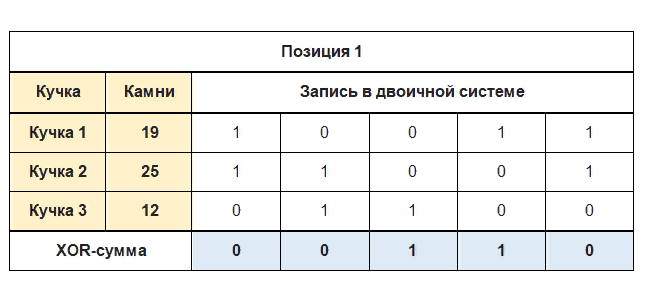
\includegraphics[scale=0.6]{images/13.png}
\end{center}

Позиция $1$ выигрышна для $1$ игрока, поскольку \textsc{XOR}-сумма не равна $0$. 

Сформируем правильный ход игрока. Старший ненулевой разряд XOR-суммы – это третий разряд. Рассмотрим одну из кучек, у которых в третьем разряде стоит 1. В нашем случае это единственная кучка 3. Оставляем в этой кучке 10 камней (поразрядно изменяем двоичную запись кучки 3 или же вычисляем XOR-сумму двух строк: строки кучки 3 и итоговой нижней строки), то есть забираем 2 камня.

Второй игрок как-то ходит, но он находится в нулевой сумме, первый игрок его всегда туда переводит, поэтому он и выиграет игру.

\end{proof}

\textbf{Следствие теоремы.} Любое состояние НИМ-игры можно заменить эквивалентным состоянием, состоящим из единственной кучки размера, равного XOR-сумме размеров кучек в старом состоянии.

Иными словами, при анализе НИМ с несколькими кучками можно посчитать XOR-сумму их размеров, и перейти к анализу НИМ из единственной кучки этого размера. Как показывает только что доказанная теорема, выигрышность/проигрышность от этого не изменится.

\begin{definition}
  \textbf{Теория Шпрага-Гранди} — это теория, описывающая так называемые \textit{равноправные игры двух игроков}, то есть игры, в которых разрешённые ходы и выигрышность/проигрышность зависят только от состояния игры. От того, какой именно из двух игроков ходит, \textit{не зависит ничего:} то есть игроки полностью равноправны.
\end{definition}

Кроме того, предполагается, что игроки располагают всей информацией (о правилах игры, возможных ходах, положении соперника).

Предполагается, что игра конечна, то есть при любой стратегии игроки рано или поздно придут в проигрышную позицию, из которой нет переходов в другие позиции. Эта позиция является проигрышной для игрока, который должен делать ход из этой позиции. Соответственно, она является выигрышной для игрока, пришедшего в эту позицию. Ничейных исходов в такой игре не бывает.

Иными словами, такую игру можно полностью описать ориентированным ациклическим графом: вершинами в нём являются состояния игры, а рёбрами — переходы из одного состояния игры в другое в результате хода текущего игрока (повторимся, в этом первой и второй игрок равноправны). Одна или несколько вершин не имеют исходящих рёбер, они является проигрышными вершинами (для игрока, который должен совершать ход из такой вершины).

Поскольку ничейных исходов не бывает, то все состояния игры распадаются на два класса: \textbf{выигрышные и проигрышные}. 

\begin{definition}
  \textbf{Выигрышные} — это такие состояния, что найдётся ход текущего игрока, который приведёт к неминуемому поражению другого игрока даже при его наилучшей игре.
\end{definition}
\begin{definition}
   \textbf{Проигрышные состояния} — это состояния, из которых все переходы ведут в состояния, приводящие к однозначной победе другого игрока.
 \end{definition}  

 Иными словами, выигрышным является состояние, из которого есть хотя бы один переход в проигрышное состояние, а проигрышным является состояние, из которого все переходы ведут в выигрышные состояния (или из которого вообще нет переходов).

 Наша задача — для любой заданной игры провести классификацию состояний этой игры, то есть для каждого состояния определить, выигрышное оно или проигрышное.

 НИМ является одним из примеров таких равноправных игр. Более того, как мы увидим чуть позже, любая из равноправных игр двух игроков на самом деле эквивалентна некоторой игре НИМ, поэтому изучение этой игры автоматически позволит нам решать все остальные игры.

\textbf{Эквивалентность любой игры НИМу. Теорема Шпрага-Гранди}

Здесь мы покажем, как любой равноправной игре двух игроков поставить в соответствие НИМ. Иными словами, любому состоянию любой игры мы научимся ставить в соответствие НИМ-кучку, полностью описывающее состояние исходной игры.

Докажем сначала важную лемму — лемму о НИМе с увеличениями.

Рассмотрим следующий модифицированный НИМ: всё так же, как и в обычном НИМе, однако теперь разрешается вместо уменьшения, наоборот, увеличить размер кучки. Ход игрока теперь заключается в том, что он либо забирает какое-то количество камней из какой-нибудь кучки, либо увеличивает размер какой-либо кучки (в соответствии с некими правилами).

Правила, по которым игрок может совершать увеличения, не важны, конкретные правила увеличений в доказательстве леммы никак не используются. Однако игра должна оставаться ацикличной, так что какие-то правила всё же должны быть.

\begin{lemma}
  Лемма о НИМе с увеличениями

  НИМ с увеличениями эквивалентен обычному НИМу в том смысле, что выигрышность или проигрышность состояния определяется по теореме Бутона согласно XOR-сумме размеров кучек.
\end{lemma}
\begin{proof}
  Идея доказательства, как и в теореме Бутона — в наличии симметричной стратегии. Мы покажем, что увеличения ничего не меняют, поскольку после того, как один из игроков прибегнет к увеличению, другой сможет симметрично ответить ему.

  В самом деле, предположим, что текущий игрок совершает ход – увеличение какой-либо кучки. Тогда его соперник может ответить ему, уменьшив обратно эту кучку до старого значения — ведь обычные ходы НИМа могут использоваться по-прежнему.

  После такого ответа игра вернётся обратно к тем же размерам кучек, то есть игрок, совершивший увеличение, ничего от этого не выиграет. Так как игра ациклична, то рано или поздно ходы-увеличения кончатся, и текущему игроку придётся делать ход-уменьшение, а это и означает, что наличие увеличивающих ходов не меняет ровным счётом ничего.
\end{proof}

Перейдём теперь к самому главному в данном рассуждении факту — теореме об эквивалентности любой равноправной игры двух игроков некоторому НИМу.

\begin{theorem}
  Теорема Шпрага-Гранди

  Рассмотрим любое состояние $v$ некоторой равноправной игры двух игроков. Пусть из него есть переходы в некоторые состояния $v_i, i=1,2,\ldots,k \qquad k \geq 0$. 

  Утверждается, что состоянию $v$ этой игры можно поставить в соответствие кучку НИМА некоторого размера $x$ (которая будет полностью описывать состояние $v$ нашей игры - то есть эти два состояния будут эквивалентны). Это число $x$ называется \textbf{Значением Шпрага-Гранди} состояния $v$
\end{theorem}

Это число $x$ можно находить следующим образом. Посчитаем значение Шпрага-Гранди $x_i$ по каждому переходу $(v,v_i)$ и положим:
$$x = \operatorname{mex}(x_1,\ldots,x_k)$$
где $\operatorname{mex}$ - функция от множества неотрицательных чисел, которая возвращает неотрицательное число, не встречающееся в этом множестве ("minimum excludant").

Таким образом, мы можем, стартуя от вершин без исходящих рёбер, постепенно посчитать значения Шпрага-Гранди для всех состояний нашей игры. Если значение Шпрага-Гранди состояния равно нулю, то это состояние проигрышно, иначе — выигрышно.

\begin{proof}
    Будем доказывать теорему по индукции.

    Для вершин, из которых нет ни одного перехода, величина $x$ будет получаться как $\operatorname{mex}$ от пустого множества, то есть $x=0$. В самом деле, состояние без переходов — это проигрышное состояние, и ему действительно должна соответствовать НИМ-кучка размера 0.

    Рассмотрим теперь любое состояние $v$, из которого есть переходы. По индукции мы можем считать, что для всех состояний $v_i$, в которые мы можем перейти из текущего состояния $v$, значения $xi_$ уже подсчитаны.

    Посчитаем величину $p = \operatorname{mex}(x_1,\ldots,x_k)$. Тогда, согласно определению функции $\operatorname{mex}$, мы получаем, что для любого числа $i$ в промежутке $[0,p)$ найдется хотя бы один соответствующий переход из состояний $v_i$. Кроме того, могут существовать также дополнительные переходы - в состояния со значениями, большими $p$.

    Это означает, что текущее состояние эквивалентно состоянию НИМа с увеличениями с кучкой размера $p$: в самом деле, у нас есть переходы из текущего состояния в состояния с кучками всех меньших размеров, а также могут быть переходы в состояния больших размеров.

  Следовательно, величина действительно является искомым значением Шпрага-Гранди для текущего состояния, что и требовалось доказать.
\end{proof}



\newpage
\subsection{Биматричные игры. Решение в чистых и смешанных стратегиях}

\begin{definition}
  \textbf{Биматричная игра} – это матричная игра двух лиц, каждый из которых при выборе стратегии руководствуется своей платежной матрицей. Каждый игрок стремится максимизировать свой выигрыш. 

  Интересы игроков могут быть различны, но, в отличие от антагонистической игры, не прямо противоположны. Другими словами, сумма выигрышей может быть не равна $0$.
\end{definition}

При анализе биматричных игр мы сохраним две гипотезы, действительные и при анализе антагонистических игр: гипотезу о полной информированности игроков и гипотезу об их рациональном поведении.

Согласно гипотезе о \textbf{полной информированности игроков}, каждому игроку до начала игры
\textit{известны все его собственные стратегии, все стратегии другого игрока}, а также его собственная
\textit{функция выигрыша и функция выигрыша другого игрока}. 

Таким образом, не известной в игре
является лишь то, какую конкретную стратегию выберет другой игрок из известного обоим
множества его допустимых стратегий.

\textbf{Гипотеза о рациональном поведении} утверждает, что поведение игроков полностью задается
\textit{функцией выигрыша.} Каждый игрок стремится \textit{максимизировать свою функцию выигрыша} и из
разных исходов выберет тот, который дает ему больший выигрыш.

Обе гипотезы ограничивают применимость моделей. Игрокам зачастую не вполне известны не только возможные стратегии противника, но даже и свои собственные стратегии. Оценки выигрыша размыты и формализовать их не так просто. Игроки могут действовать импульсивно, подчиняясь эмоциям, а не рациональным выводам. Тем не менее, сформулированные гипотезы
позволяют моделировать и анализировать конфликтные ситуации относительно простыми средствами и получать исчерпывающие модельные ответы.

Обозначим матрицу выигрышей первого игрока посредством $A: m \times n$, второго - $B: m \times n$. Первый игрок имеет $m$ чистых стратегий, а второй $n$ чистых стратегий. В результате выбора $i$-ой стратегии $1$-ым игроком и $j$-й стратегии вторым игроком, первый игрок получает выигрыш $a_{ij}$, а второй игрок $b_{ij}$.

Если $A+B=0$, то игра антагонистическая. При задании биматричной игры не предполагается связь матриц, в анализе участвуют обе матрицы.

Решение антагонистической игры в чистых стратегиях может не существовать, а в смешанных существует всегда. Решение биматричных игр мы будем искать сразу в смешанных стратегиях.

Ситуация, как и антагонистической игре, задается парой смешанных стратегий игроков, парой векторов $P$ и $Q$:
$$P = (p_1,\ldots,p_m) \qquad Q = (q_1,\ldots,q_n)$$
$$\sum\limits_{i=1}^m p_i = 1 \qquad \sum\limits_{j=1}^n q_i = 1 \qquad p_i,q_j \geq 0$$

Частный случай смешанной стратегии, когда одна компонента $1$, а остальные равны $0$, соответствует выбору \textit{чистой стратегии} - конкретной строки или столбца.

Предположим, игроки выбрали какие-то смешанные стратегии $P$ и $Q$. Результатом игры считается математическое ожидание величины выигрыша. 

Для первого игрока - $E_1 = PAQ^T$, для второго $E_2 = PBQ^T$. 

\begin{definition}
  Ситуация, приемлемая для обоих игроков, называется ситуацией \textit{равновесия по Нэшу} и является решением игры, образующие эту ситуацию стратегии называются \textit{оптимальными}.
\end{definition}

Стратегии $P^*$ и $Q^*$ оптимальны, если они приемлемы для обоих игроков, то есть выполнены оба неравенства:
$$PAQ^{*T} \leq P^*AQ^{*T} \qquad P^*BQ^{T} \leq P^*BQ^{*T}$$

Поняти решения биматричной игры обобщает понятие решения, введенное ранее для антагонистических игр.

\subsubsection{Решение биматричных игр 2x2}

Будем рассматривать $2\times 2$ биматричную игру с матрицами выигрышей:
$$A = \begin{bmatrix}
  a_{11} & a_{12} \\
  a_{21} & a_{22}
\end{bmatrix}, \qquad B = \begin{bmatrix}
  b_{11} & b_{12} \\
  b_{21} & b_{22}
\end{bmatrix}$$

Матрица $A$ описывает выигрыши первого игрока, $B$ - второго. Смешанные стратегии игроков полностью описываются в этом частном случае вероятностью применения своей первой стратегии каждым из игроков, то есть:
$$P = (p,1-p) \qquad Q = (q,1-q)$$

Поскольку $0 \leq p,q \leq 1$, то каждая ситуация в смешанных стратегиях в $2 \times 2$ биматричной игре может быть изображена точкой на единичном квадрате на плоскости $(p,q)$.

Идея нахождения решения игры состоит в следующем: мы опишем множества приемлемых ситуаций для каждого из игроков, затем нарисуем эти множества на единичном квадрате и графически найдем их пересечение. Очевидно, найденное решение (или множество решений) является равновесием по Нэшу.

\textbf{Определение ситуации равновесия по Нэшу}

Начнем с первого игрока. Игровая ситуация $(P,Q)$. 

Математическое ожидание $\mathbb{E}$ выигрыша первого игрока при выборе игроками своих смешанных стратегий $P$ и $Q$, то есть при выборе величин $p$ и $q$, есть:
$$ \mathbb{E}(p,q) = PAQ^T = pqa_{11} + p \cdot (1-q)a_{12} + (1-p)qa_{21} + (1-p)(1-q)a_{22} $$
$$\mathbb{E}(p,q) = (a_{11}-a_{12}-a_{21}+a_{22})pq + (a_{12}-a_{22})p + (a_{21}-a_{22})q + a_{22}$$

Для того, чтобы стратегия $P$ была оптимальной, необходимо, чтобы она была не хуже каждой из двух чистых стратегий  то есть необходимо, чтобы выполнялись неравенства:
$$\left \{
\begin{matrix}
 qa_{11} + (1-q)a_{12} \leq \mathbb{E}(p,q)   \\
qa_{21} + (1-q)a_{22} \leq \mathbb{E}(p,q)  
\end{matrix} \right .$$

Если подставить в этим выражения математическое ожидание и упростить, то получатся следующие неравенства:
$$(a_{11}-a_{12}-a_{21}+a_{22})(1-p)q+(a_{12}-a_{22})(1-p) \leq 0$$
$$(a_{11}-a_{12}-a_{21}+a_{22})pq + (a_{12}-a_{22})p \geq 0$$

Если ввести обозначения, что $C=a_{11}-a_{12}-a_{21}+a_{22}$ и $\alpha = a_{22} - a_{12}$, то условие приемлемости принимает вид:
$$C(1-p)q - \alpha(1-p) \leq 0$$
$$Cpq -\alpha p \geq 0$$

Рассмотрим $3$ частных случая:

\begin{enumerate}
  \item $(p,q)=(1,q)$, в этой ситуации первый игрок выбирает свою первую стратегию. Первое равенство выполняется, значит ситуация будет приемлемой для первого игрока в том случае, если:
  $$Cq-\alpha \geq 0 $$
  $$\begin{cases}
    q \geq \frac{\alpha}{C}, C>0 \\
    q \leq \frac{\alpha}{C}, C<0
  \end{cases}$$

  \item $(p,q) = (0,q)$, в этой ситуации первый игрок выбирает свою вторую стратегию. Второе неравенство выполняется, а оставшееся имеет вид:
  $$\begin{cases}
    q \leq \frac{\alpha}{C} , C > 0\\
    q \geq \frac{\alpha}{C}, C < 0 
  \end{cases}$$

  \item $p \neq 0$, тоогда можно поделить равенства на $1-p$ и на $p$, тогда:
  $$q = \frac{\alpha}{C}$$
\end{enumerate}

\begin{center}
  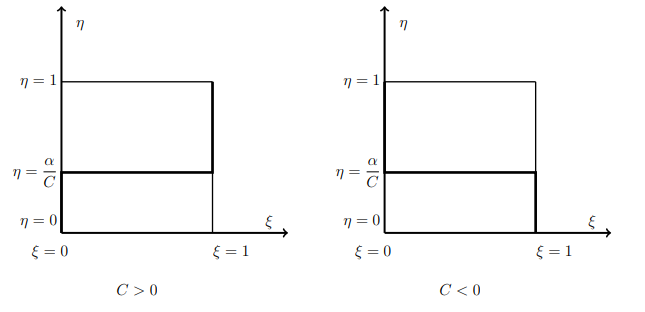
\includegraphics[scale=0.6]{images/6.png}

  Рис. 6: Биматричные игры $2\times2$: множество приемлемых стратегий для первого игрока
\end{center}

Заметим, что зигзаг может быть и вырожденным. Если $C=0$ и $\alpha \neq 0$, то реализуются только первые две ситуации и множество распадается на два отрезка. Если $C=0$ и $\alpha=0$, то \textbf{любая допустимая ситуация будет приемлемой для первого игрока} (матрица выигрыша состоит из одинаковых строк и выигрыш становится бесмысленным).

Аналогичные размышления можнопривести и для второго игрока, но можно поступить проще и заменить матрицу $A$ на $B^T$, поскольку мы полагаем, что стратегиям первого игрока соответствуют строки матрицы, а второго - столбцы.

Выполнив замеу, получим следующий результат: множество приемлемых для второго игрока ситуаций определяется двумя параметрами:
$$D = b_{11}-b_{12}-b_{21}+b_{22}$$
$$\beta = b_{22}-b_{21}$$

Нарисуем это множество:
\begin{center}
  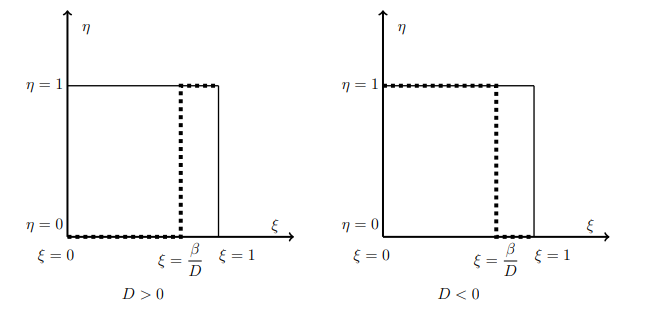
\includegraphics[scale=0.6]{images/7.png}

  Рис. 7: Биматричные игры $2\times2$: множество приемлемых стратегий для второго игрока
\end{center}

Совместим теперь эти множества на одном риуснке. В зависимости от знаков величин $C$ и $D$ возможны четыре ситуации:
\begin{center}
  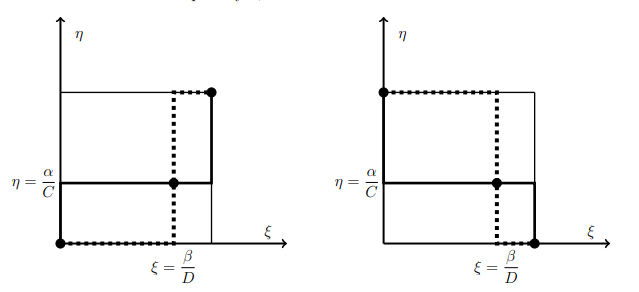
\includegraphics[scale=0.6]{images/8.png}

  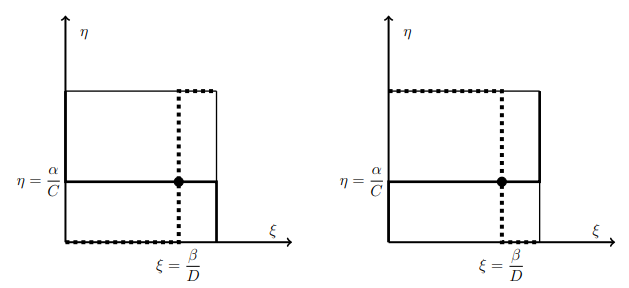
\includegraphics[scale=0.6]{images/9.png}
\end{center}

Точек равновесия может быть либо $3$, либо одна. Кроме того, если один или оба зигзага вырождены, возможно бесконечное число равновесных ситуаций.

Рассмотрим несколько примеров биматричных игр $2\times 2$.

\subsubsection{Игра Семейный спор и ее анализ на языке биматричных игр}

Семейная пара, муж и жена, выбирают, что им посмотреть по телевизору: муж хочет смотреть по телевизору футбол, а жена - сериал. У каждого игрока имеется две стратегии, игра описывается матрицами $A$ и $B$, где $A$ - матрица мужа, а $B$ - матрица жены.

У обоих игроков первая стратегия - посмотреть футбол, а вторая - посмотреть сериал.
$$A = \begin{bmatrix}
  2 & -1 \\
  -1 & 1 
\end{bmatrix} \qquad B = \begin{bmatrix}
  1 & -1 \\
  -1 & 2 
\end{bmatrix}$$

Оба -  и муж и жена - предпочтут уступить, лишь бы посмотреть передачу вместе, то есть игрокам выгоднее быть вместе, чем врозь. Но выбор неравнозначен, возможно, им стоит предварительно обсудить ситуацию и о чем-то договориться. Для антагонистических игр это не имеет смысла. Таким бразом, \textit{в биматричных играх модет быть смысл в предварительной договоренности}, а в антагонистических нет, так что биматричные игры обладают свойствами, которыми антагонистические игры не обладают.

Предположим, что оба игрока выберут смотреть футбол, возникшая ситуация будет устойчивой, это равновесие по Нэшу. Аналогично при выборе сериала. Но результаты будут разными. Таким обрамзом, в отличие от антагонистической игры, в биматричной игре разные ситуации могут дать разные выигрыи, даже при выборе чистых стратегий. А ведь есть еще и смешанные.

Можно найти гарантированный выигрыш в гарантируюищх смешанных стратегиях. Для этого каждую матрицу будем рассматривать как матрицу антагонистической игры. Получим:
$$q = \frac{\alpha}{C} = \frac{2}{5} = 0.4 \Rightarrow Q = (0.4,0.6)$$
$$p = \frac{\beta}{C} = \frac{3}{5} = 0.6 \Rightarrow P = (0.6,0.4)$$
$$E = PAQ^T = 0.2$$
выигрыш каждого равен $0.2$. 

\begin{center}
  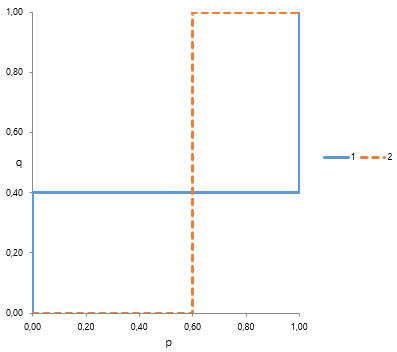
\includegraphics[scale=0.6]{images/10.png}

  Риc.8: гарантированный выигрыш в смешанных стратегиях
\end{center}

В данной игре имеется две ситуации равновесия в чистых стратегиях, когда муж и жена идут смотреть вместе либо футбол, либо балет. Но эта ситуация неравноценна для игроков.

Казалось бы, что мы получили полезный результат, однако эта ситуация не является равновесной. Но \textit{гарантируюзие смешанные стратегии для биматричной игры могут оказаться неустойчивыми}.

\subsubsection{Дилемма заключенного}

Два бандита в отдельных камерах ожидают суда по подозрению в тяжком преступлении.

Прокурор, имея доказательства в совершении подозреваемыми незначительного проступа (1 год тюрьмы), предлагает каждому из бандитов признаться в совершении тяжкого преступления.

За признание обещано освободить из тюрьмы, но напарник будет осужден к $20$ годам тюрьмы. Если признаются оба бандита, то получат по $5$ тюрьмы.

В данной игре участвуют $2$ игрока: $1$ - это бандит $1$, игрок $2$ - бандит $2$.

Их выигрыши представлены в следующей таблице:
$$A = \begin{bmatrix}
  -5 & 0 \\ 
  -20 & -1
\end{bmatrix} \qquad B = \begin{bmatrix}
  -5 & -20 \\ 
  0 & -1
\end{bmatrix}$$
где первые строки и столбцы - стратегия признаться, а вторая строка и второй столбец - стратегия не признаться.

В этой игре единственная ситуация равновесия - обоим бандитам признаться и получить по пять лет тюрьмы. Данная ситуация является \textit{доминирующим равновесием}.

Это не самый лучший исход для игроков: если оба бандита не признаются, то оба получит год тюрьмы. Но такой исход не является ситуацией равновесия, поскольку у каждого из бандитов остается искушение признаться и избежать тюрьмы.

\begin{center}
  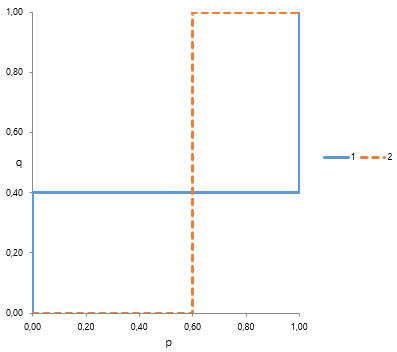
\includegraphics[scale=0.6]{images/10.png}

  Риc.9: равновесие в задаче о заключенных - доминирующее равновесие
\end{center}

\subsubsection{Графическое решение биматричных игр 2х2}

Реализация игры Семейного спора, дилеммы заключенного и антагонистических игр представлено в файле:
$$\textsc{8. биматричные игры 2x2.xlsx}$$ 


\end{document}
